\chapter[RESULTADOS]{\textbf {RESULTADOS}}

O software construído por este projeto, que está na versão 0.1, foi inteiramente construído pelo autor desta obra, e está liberado como software livre no \emph{site \url{https://github.com/rob-nn/open\_gait\_analytics}}, sob a licença \emph{Massachusetts Institute of Technology (MIT)} (ver Anexo \ref{licenca_mit}). A intenção do autor é aumentar as chances de que futuras versões do software sejam construídas, não importando se serão comerciais ou gratuitas.

O software em si é composto por dois módulos que são apresentados na Figura \ref{tela1}. O principal objetivo neste momento é atrair pesquisadores da área de análise de marcha para o software. Por isso há o módulo simulação, no qual o pesquisador poderá simular sinais.
O módulo de análise visa atender tanto a pesquisadores, quanto a profissionais da área clínica. Neste momento, o software é mais um protótipo funcional do que algo pronto para o mercado. Portanto, o uso por profissionais da área clínica não é recomendado ainda.

\begin{figure}[H]
	\centering
	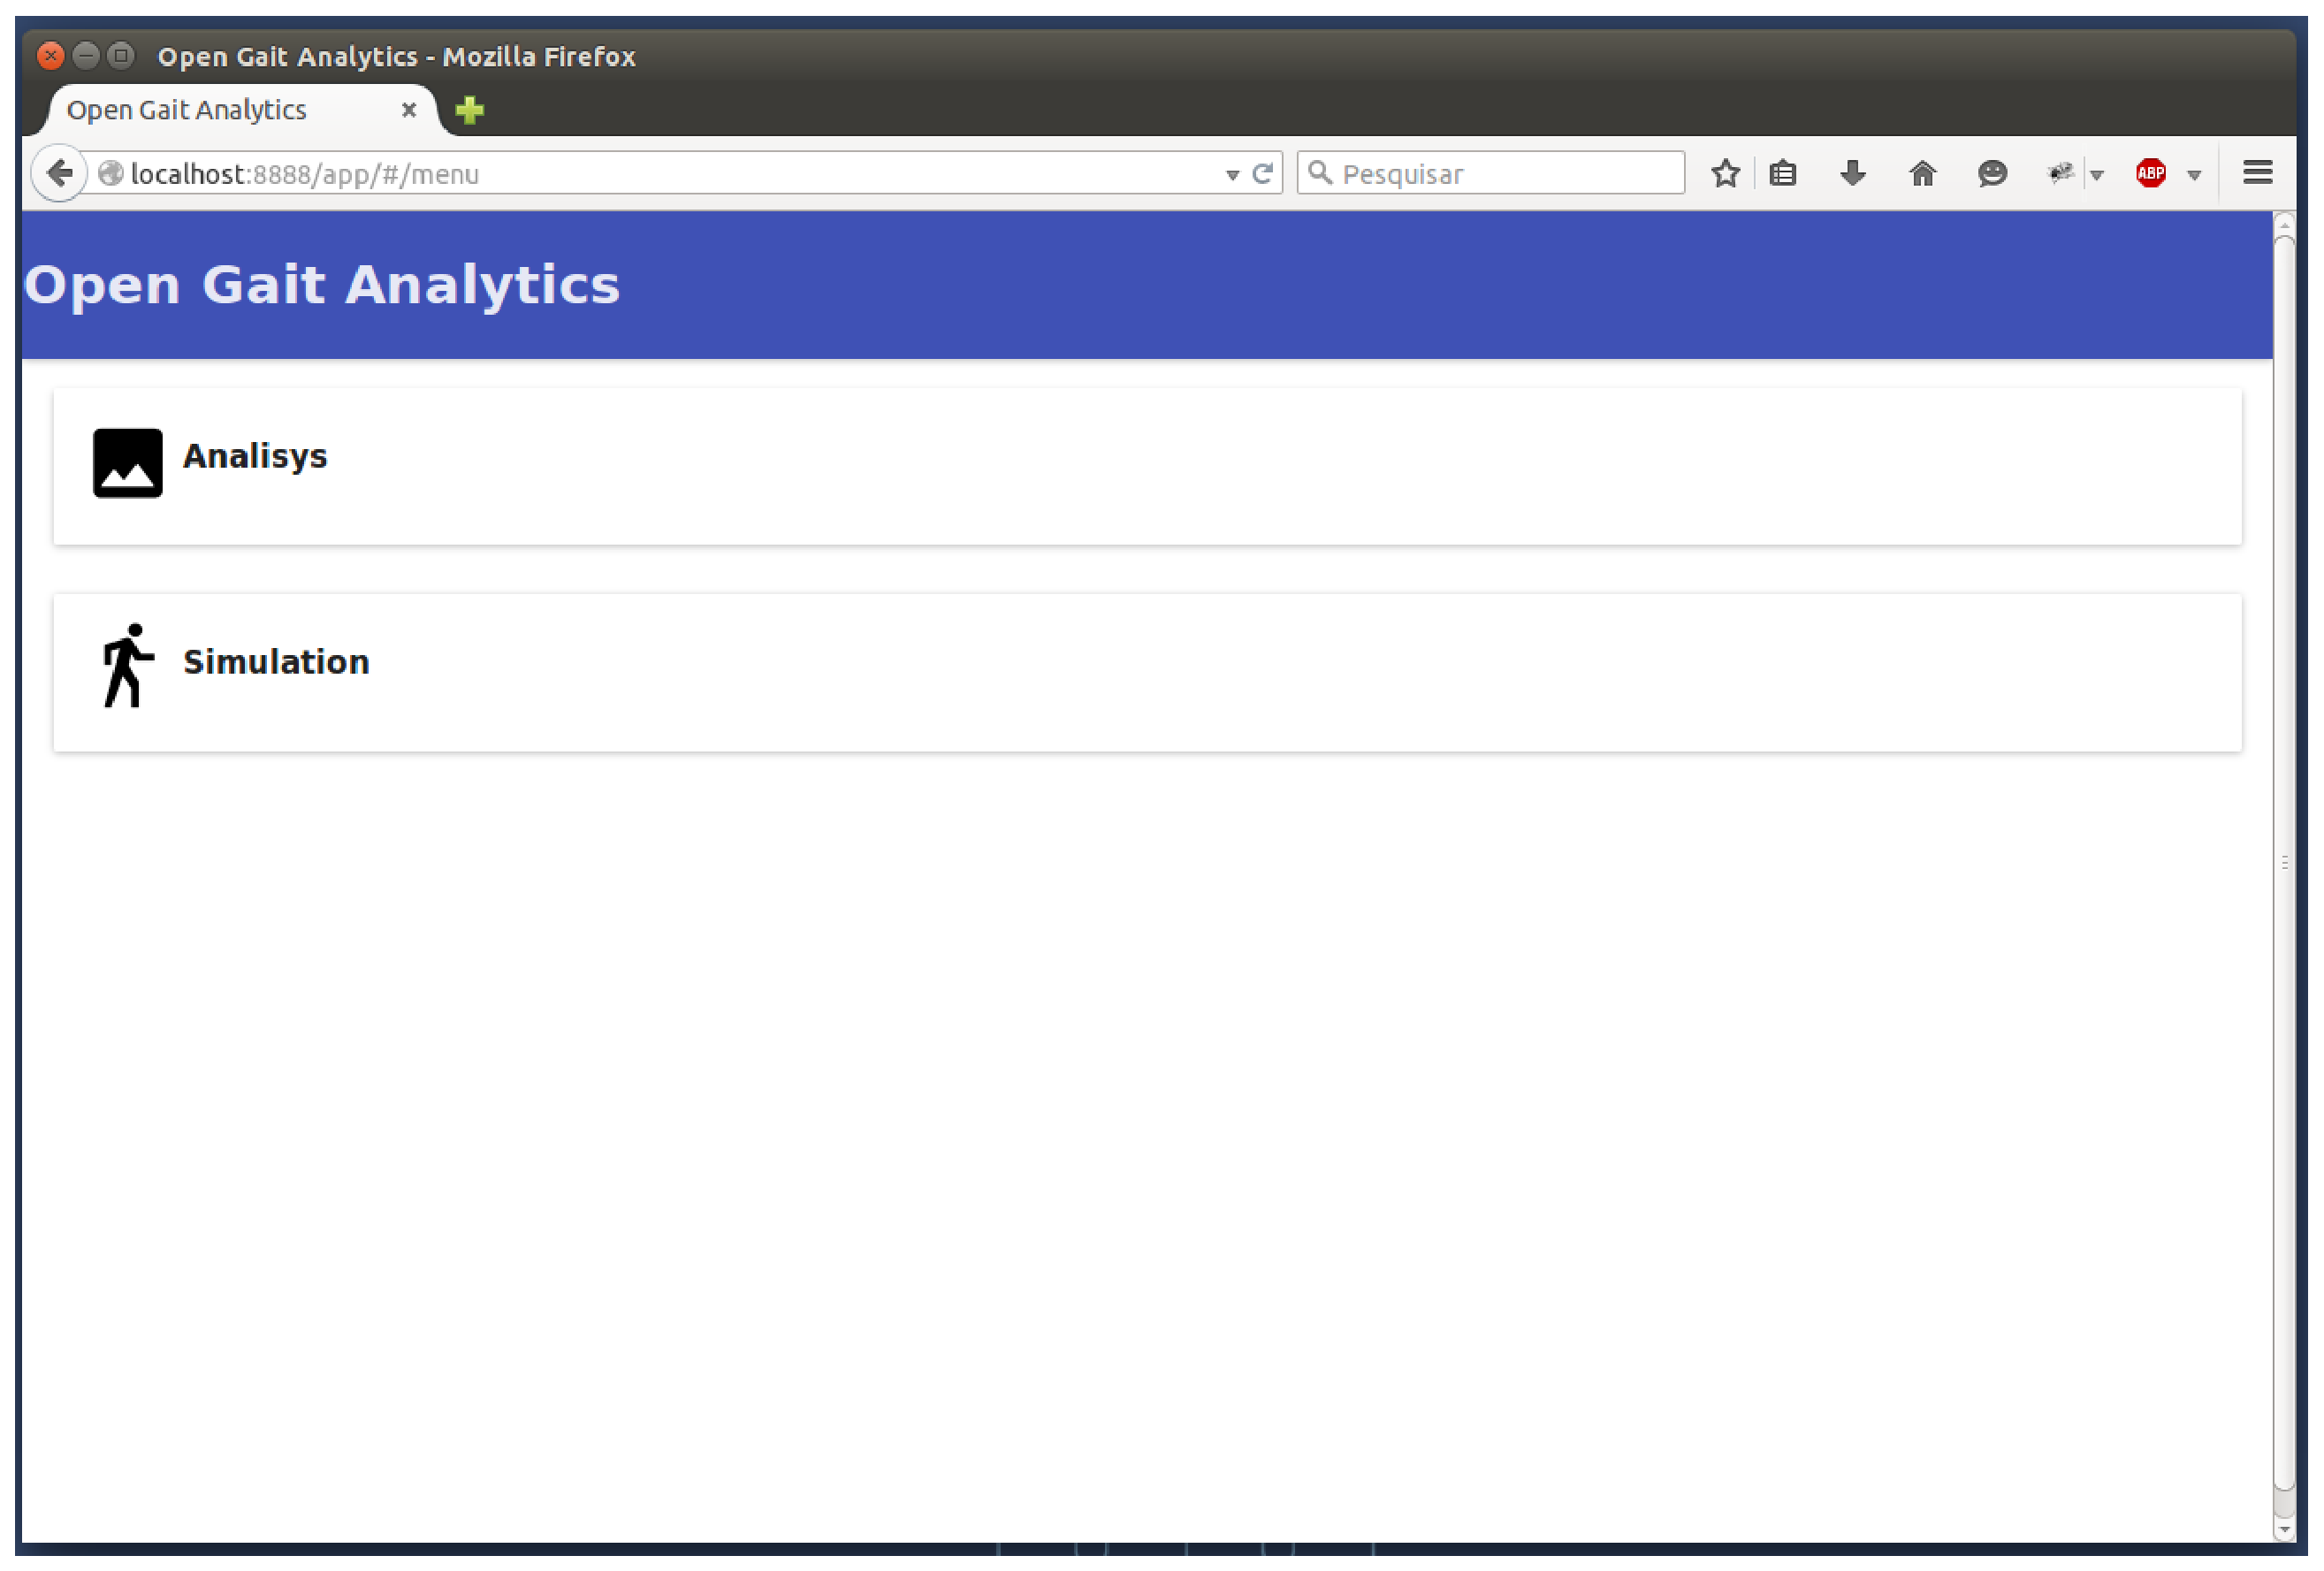
\includegraphics[width=15cm]{figuras/tela1.eps}
	\caption{Tela de seleção dos módulos.}
	\label{tela1}
\end{figure}

\section{Módulo de Análise}
Neste fase o software conta apenas com análise de movimentos, com sinais oriundos de marcadores passivos de superfície, captados por câmeras, usando o software \emph{QTM}. 
No \emph{QTM} é feita a conversão dos dados para o formato \emph{Matlab} que é reconhecido pelo sistema construído.

A primeira tela deste módulo pode ser vista na Figura \ref{tela2}. Este tela apresenta a listagem de pacientes, cadastrados no sistema. O botão abaixo a direita, é a função para adicionar novos pacientes.

\begin{figure}[H]
	\centering
	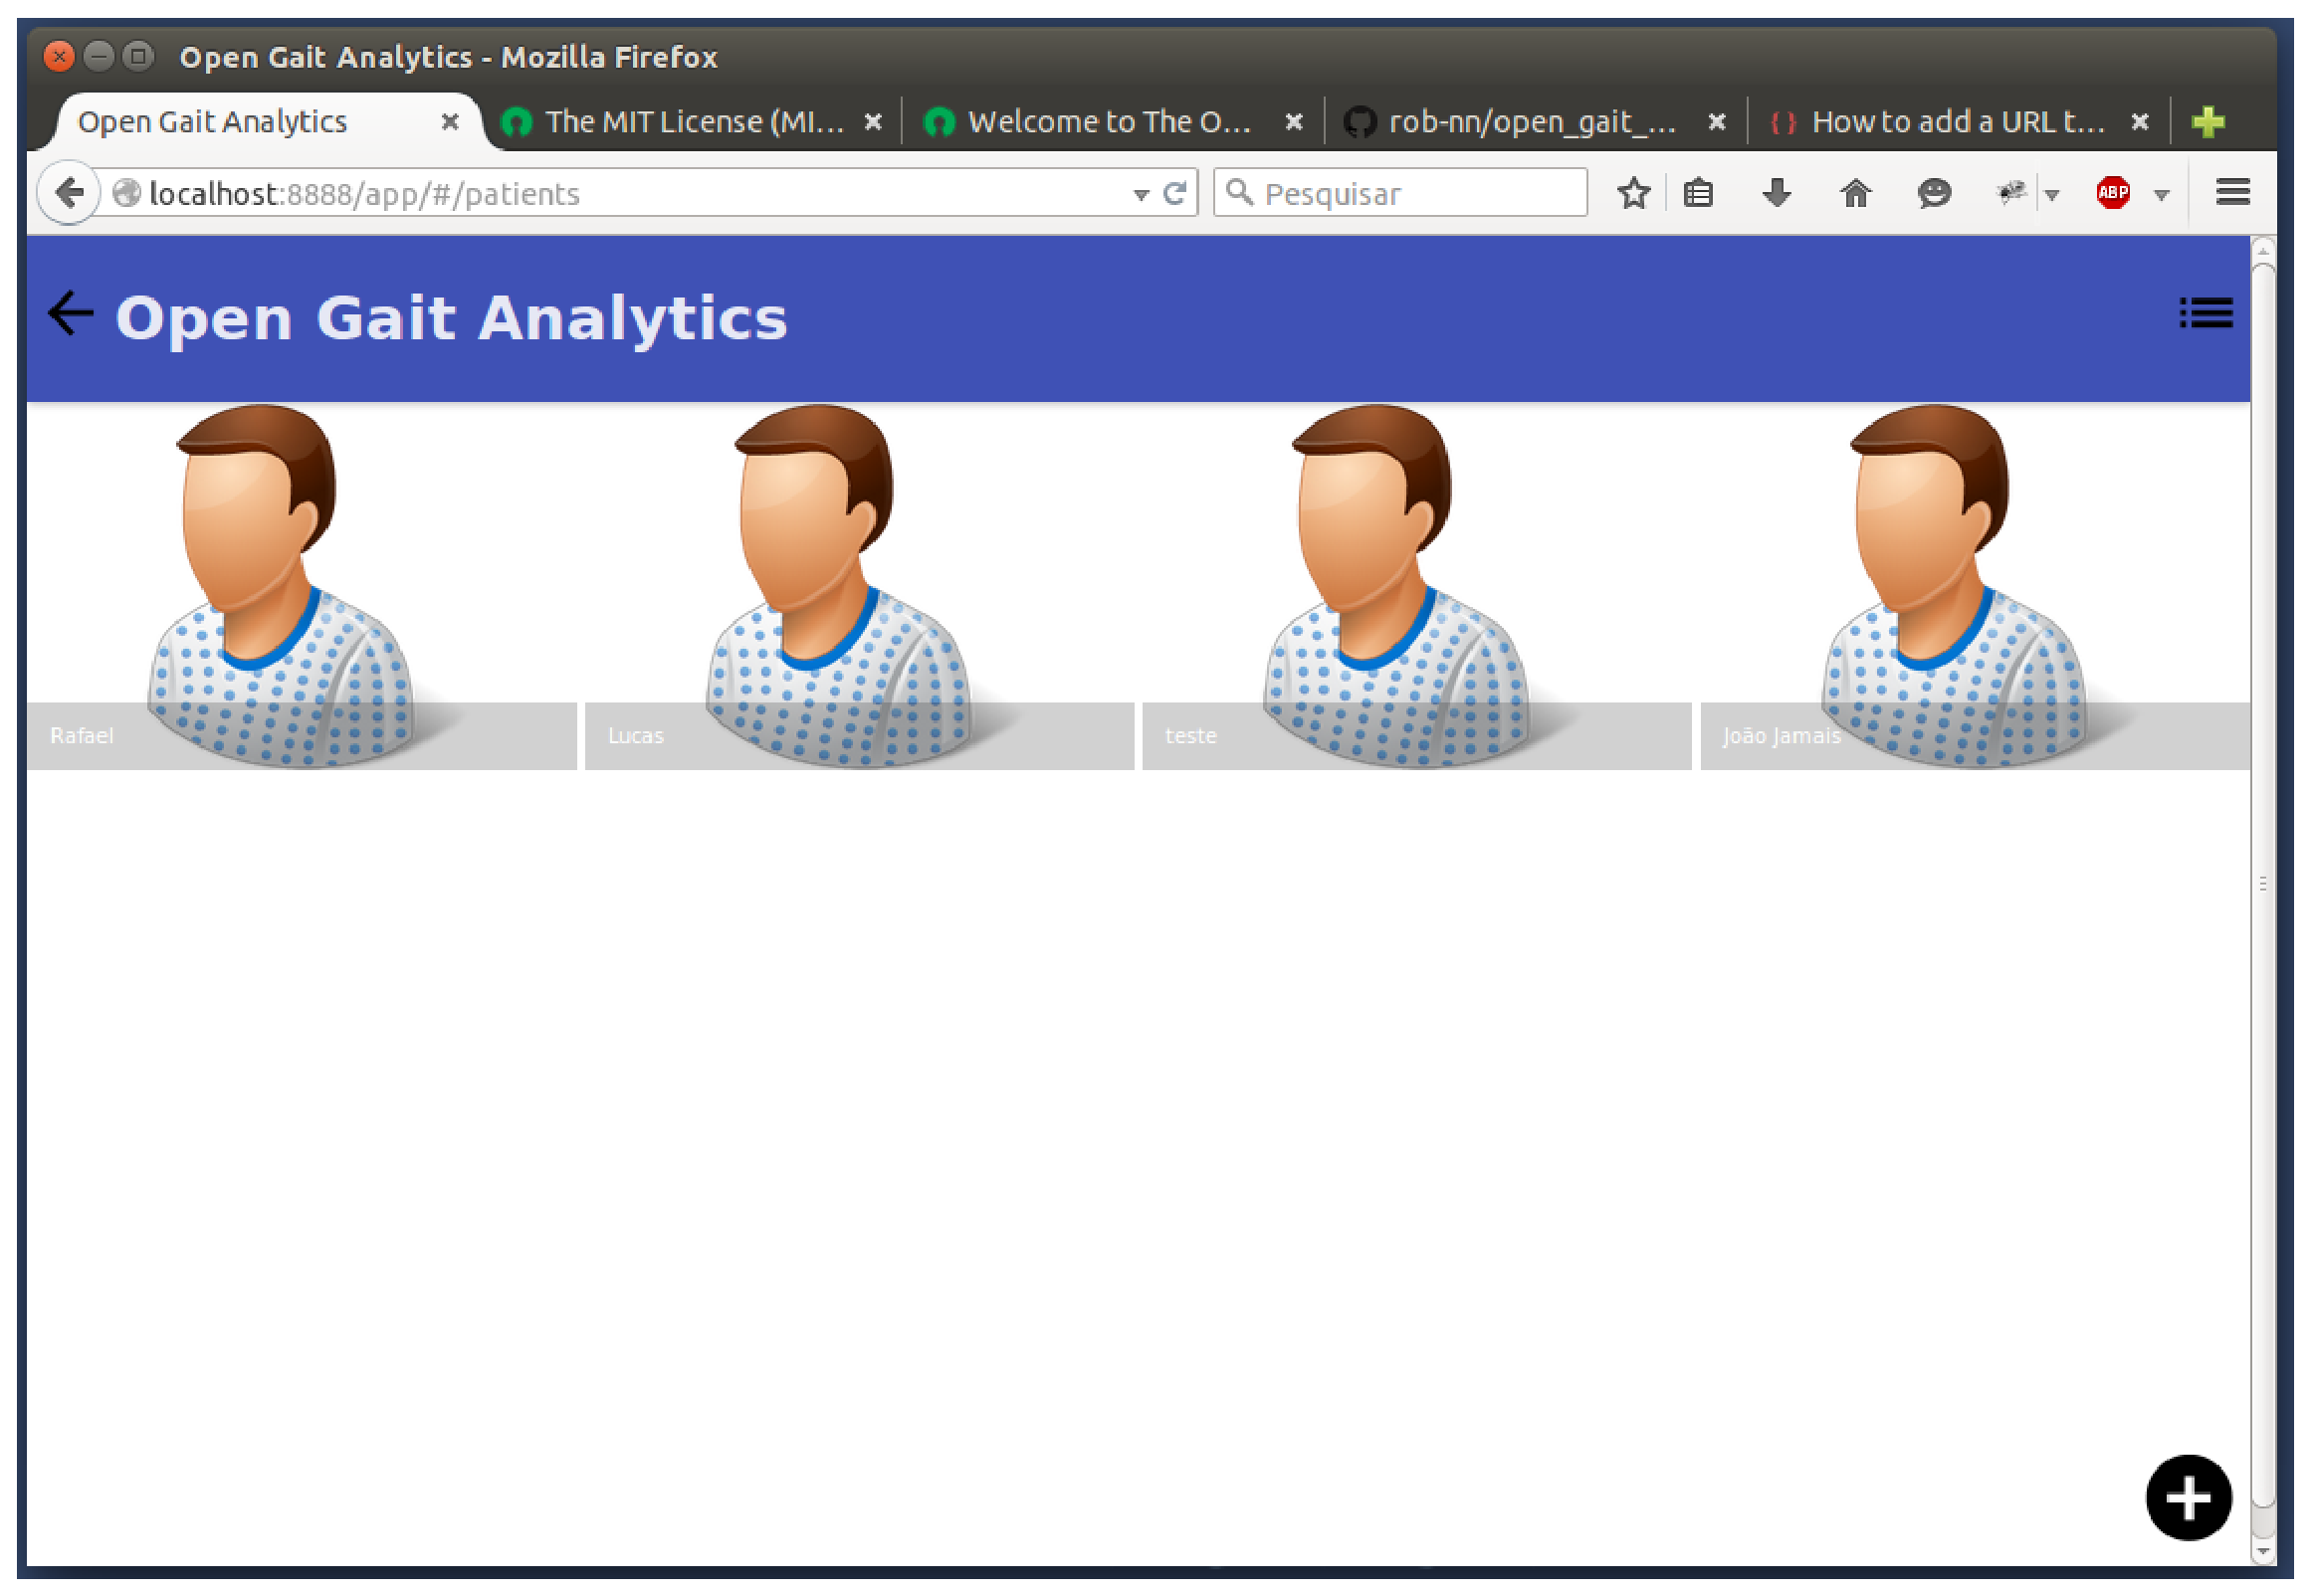
\includegraphics[width=15cm]{figuras/tela2.eps}
	\caption{Tela com a listagem de pacientes.}
	\label{tela2}
\end{figure}

A Figura \ref{tela3} mostra as informações do paciente que devem ser preenchidas ao se executar a função adicionar paciente. Esta tela é uma adaptação da ficha de avaliação que está na obra \citeonline{VeraReg}.

\begin{figure}[H]
	\centering
	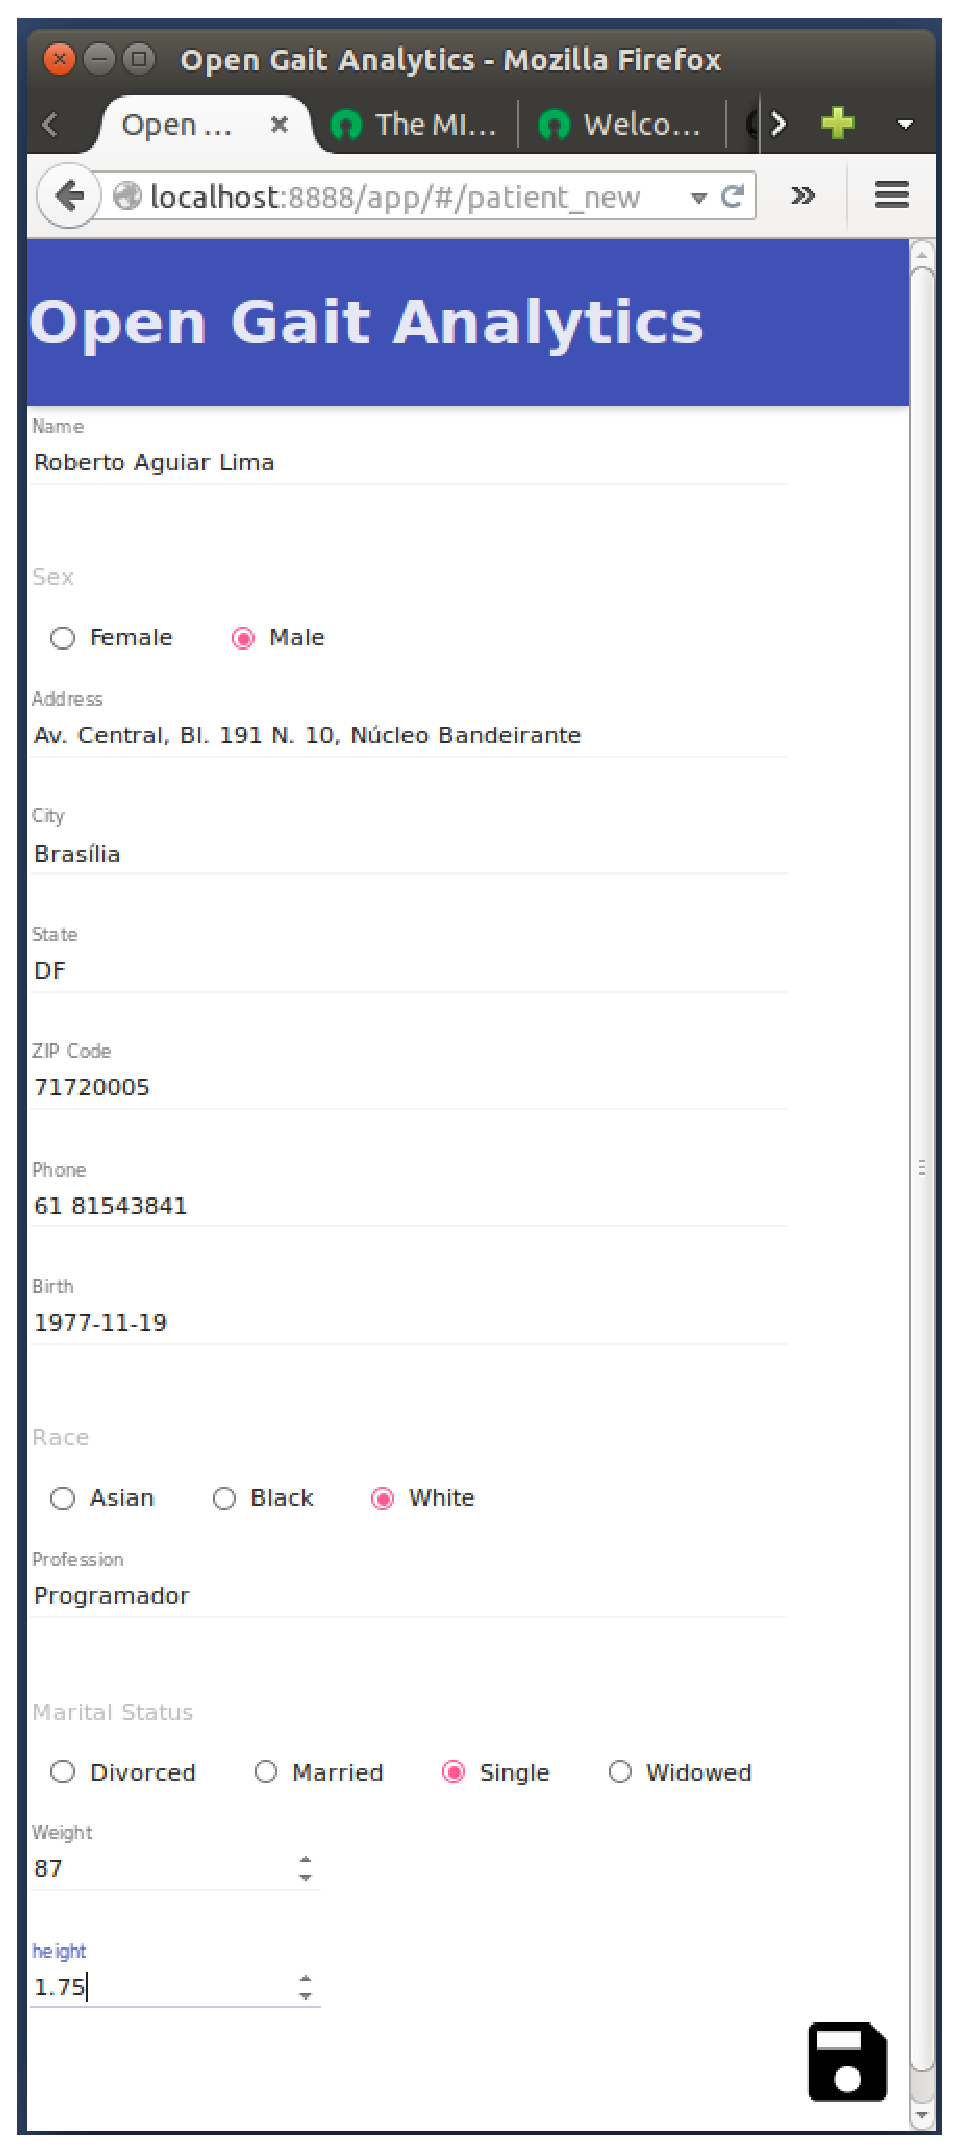
\includegraphics[width=7cm]{figuras/tela3.eps}
	\caption{Informações do paciente.}
	\label{tela3}
\end{figure}

Ao se selecionar um paciente da tela mostrada na Figura \ref{tela2}, a tela da Figura \ref{tela4} aparece. No caso em questão, nenhuma coleta de dados foi carregada para o paciente. Logo, o próximo passo é adicionar uma nova amostra de marcha.
O usuário deve então informar a descrição da coleta e a data que a mesma ocorreu e salvar estas informações, conforme a Figura \ref{tela5}.

\begin{figure}[H]
	\centering
	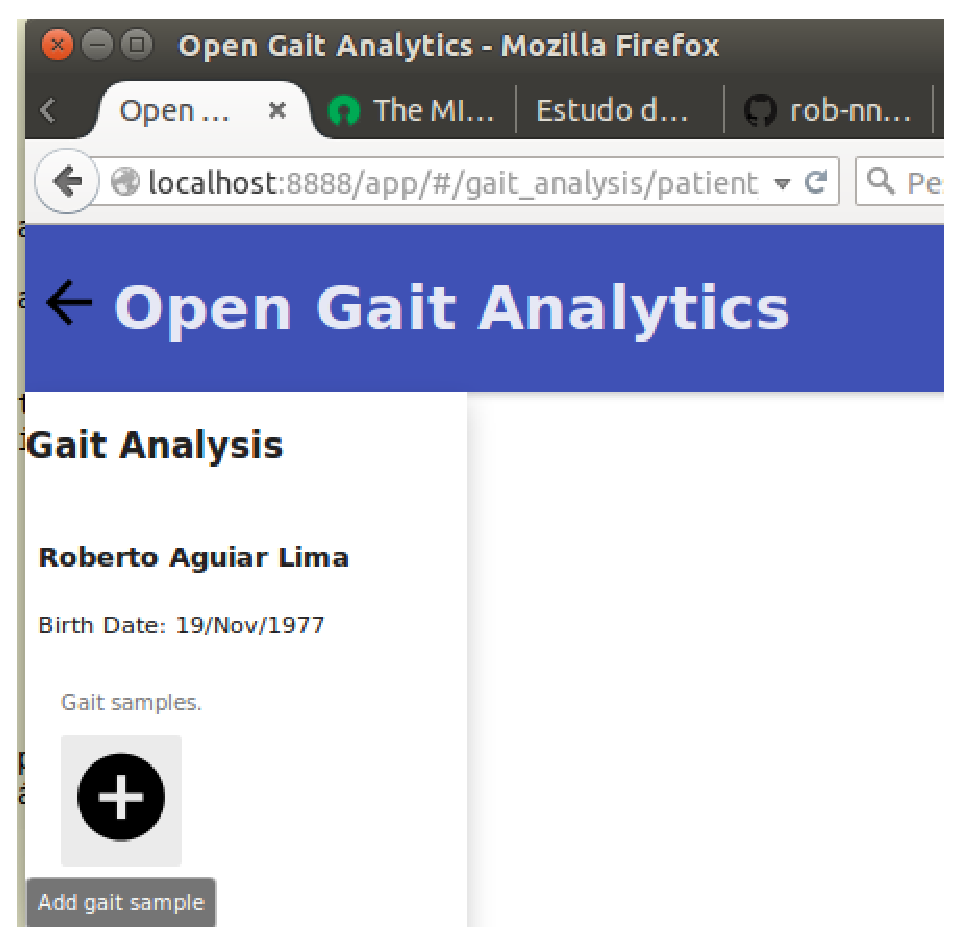
\includegraphics[width=7cm]{figuras/tela4.eps}
	\caption{Tela inicial da dados coletados do paciente.}
	\label{tela4}
\end{figure}


\begin{figure}[H]
	\centering
	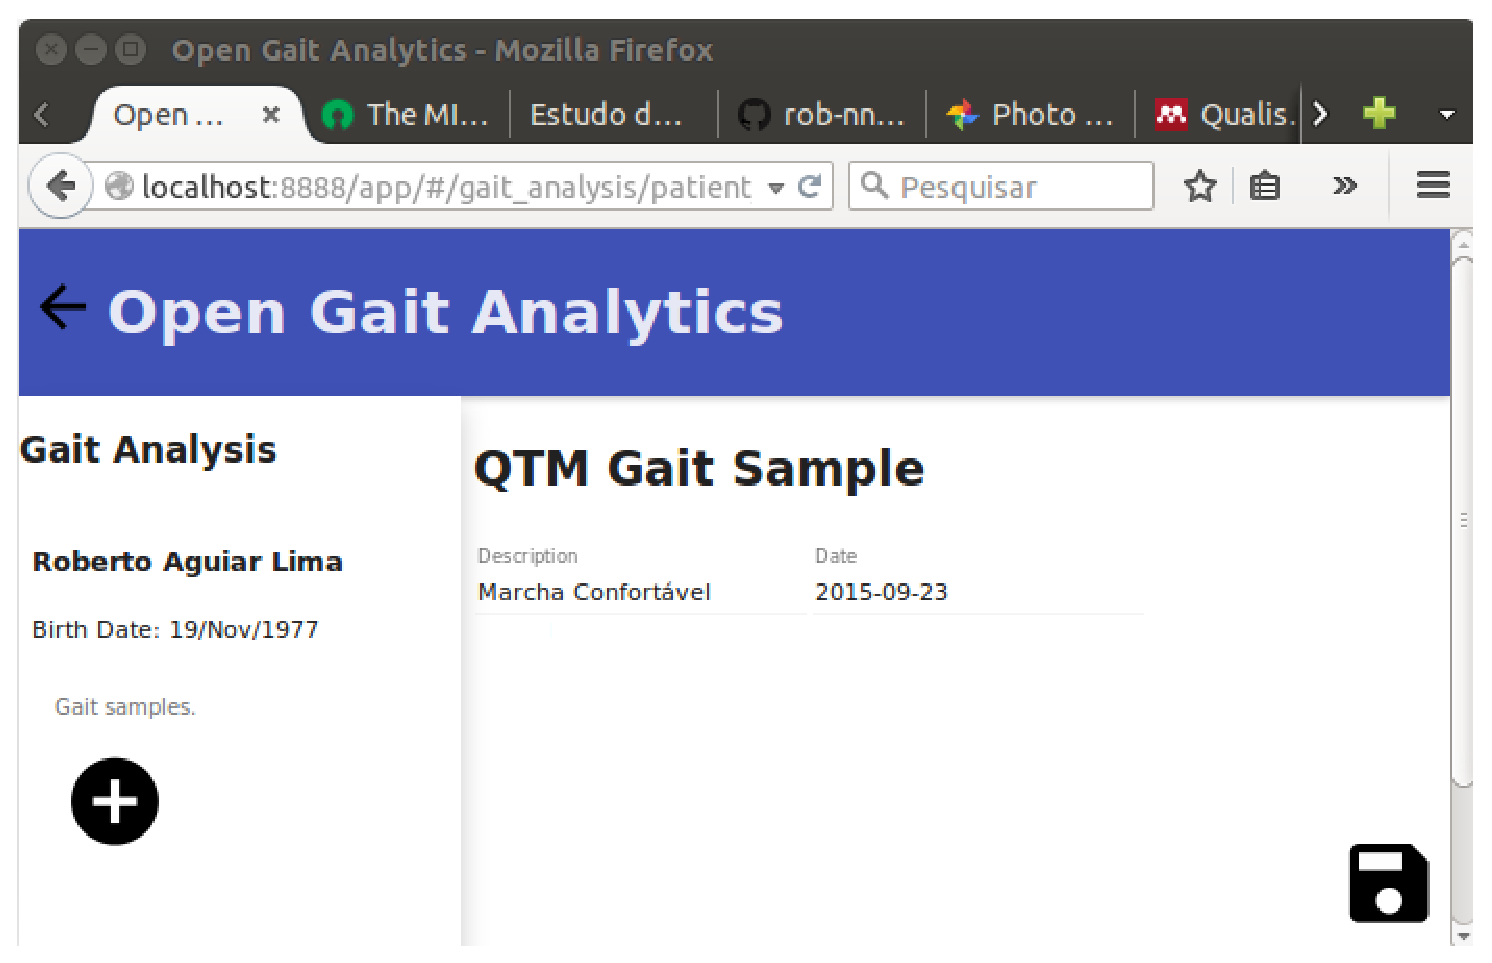
\includegraphics[width=15cm]{figuras/tela5.eps}
	\caption{Inclusão de amostra de marcha}

	\label{tela5}
\end{figure}



Depois de salva as informações o sistema pede para que o usuário selecione o arquivo proveniente do \emph{QTM}, conforme a Figura \ref{tela6}.
Depois de selecionado o arquivo com os dados da marcha, seus dados são mostrados para o usuário, conforme a Figura \ref{tela7}.

\begin{figure}[H]
	\centering
	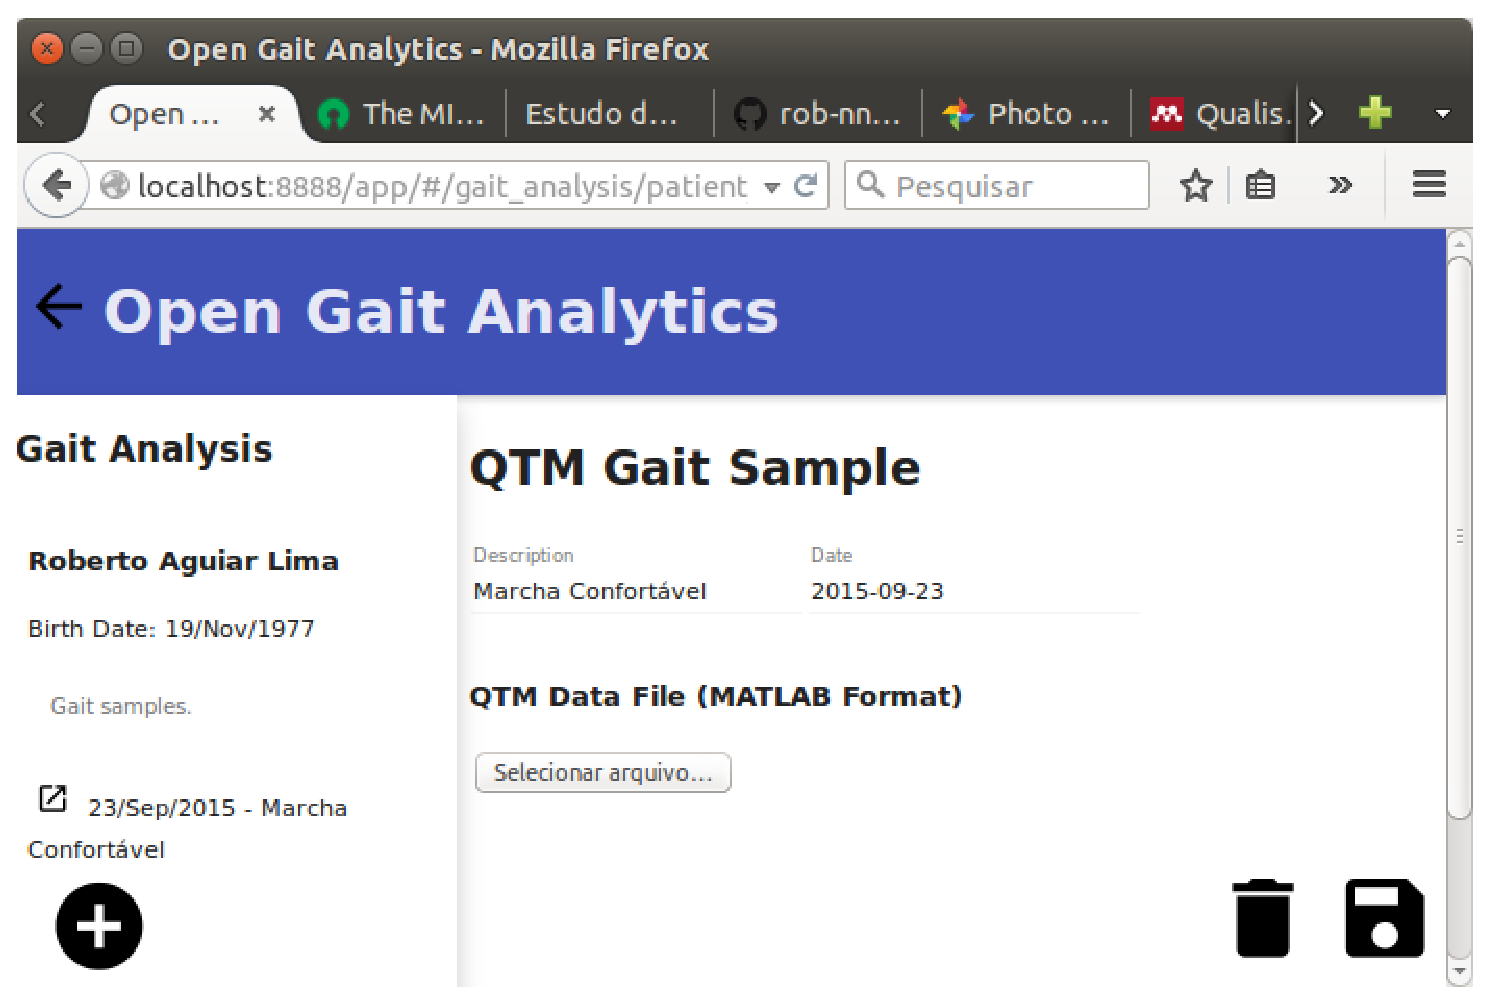
\includegraphics[width=14cm]{figuras/tela6.eps}
	\caption{Seleção do arquivo no formato \emph{MATLAB} proveniente do \emph{QTM}.}
	\label{tela6}
\end{figure}
\begin{figure}[H]
	\centering
	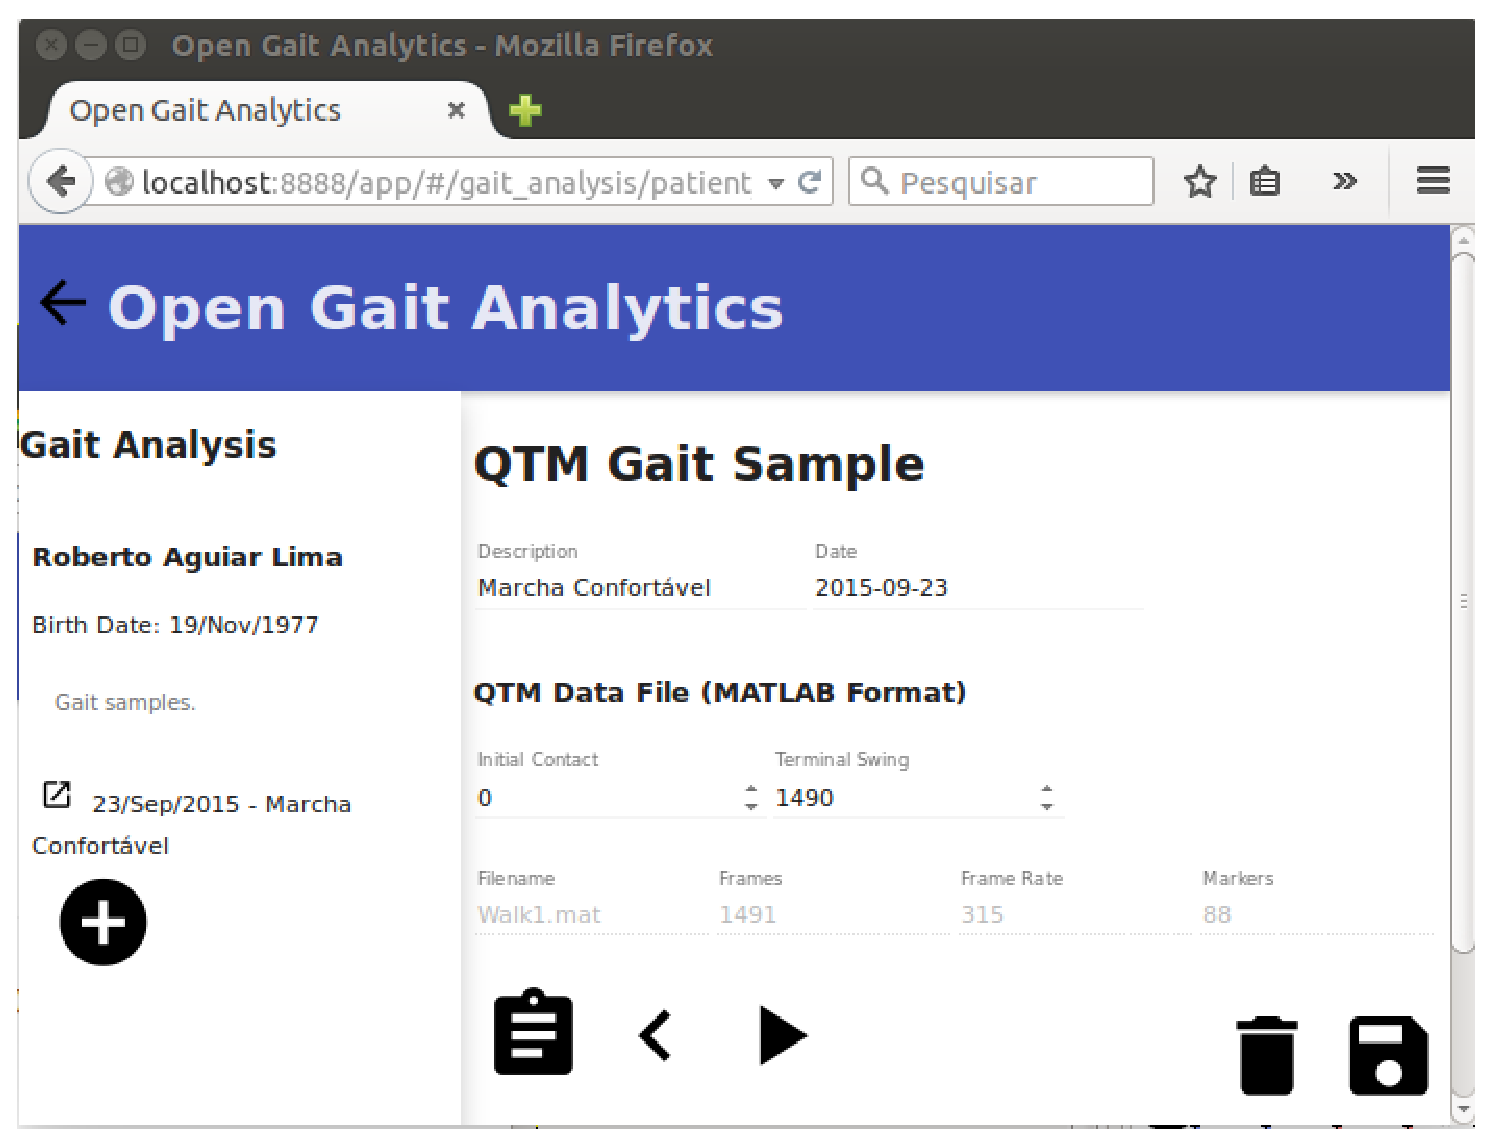
\includegraphics[width=14cm]{figuras/tela7.eps}
	\caption{Dados do arquivo provenientes do \emph{QTM}.}
	\label{tela7}
\end{figure}





Neste momento, se o usuário quiser visualizar uma animação dos dados, basta clicar na seta negra que aponta para a direita que uma animação será mostra conforme a Figura \ref{animacao1}.
Esta animação foi construída usando a tecnologia \emph{ThreeJS}, resumida na seção \ref{threejs_sec}. Uma das grandes vantagens desta característica do software em relação ao \emph{QTM}, que também a possui, é o fato de que a animação está rodando num \emph{browser web} moderno, ou seja, qualquer um com um \emph{browser} assim pode vê-la sem precisar do \emph{QTM} instalado. 
Além do mais, como o projeto pode continuar, fica a critério dos usuários decidirem que novas características seriam interessantes, não somente nas animações, mas em todo o software.


\begin{figure}[H]
  \centering
  \begin{minipage}[b]{0.32\textwidth}
    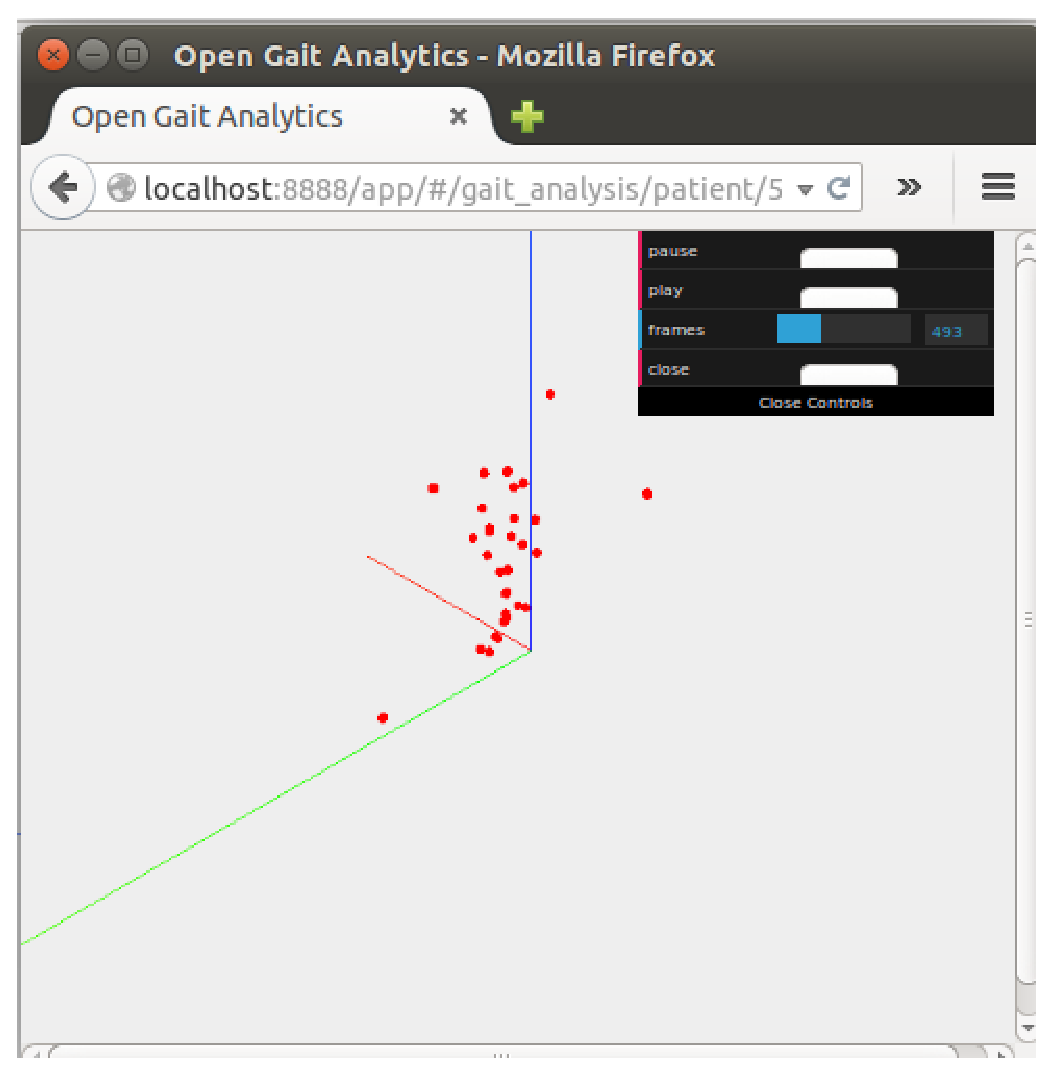
\includegraphics[width=\textwidth]{figuras/tela8.eps}
  \end{minipage}
  \hfill
  \begin{minipage}[b]{0.32\textwidth}
    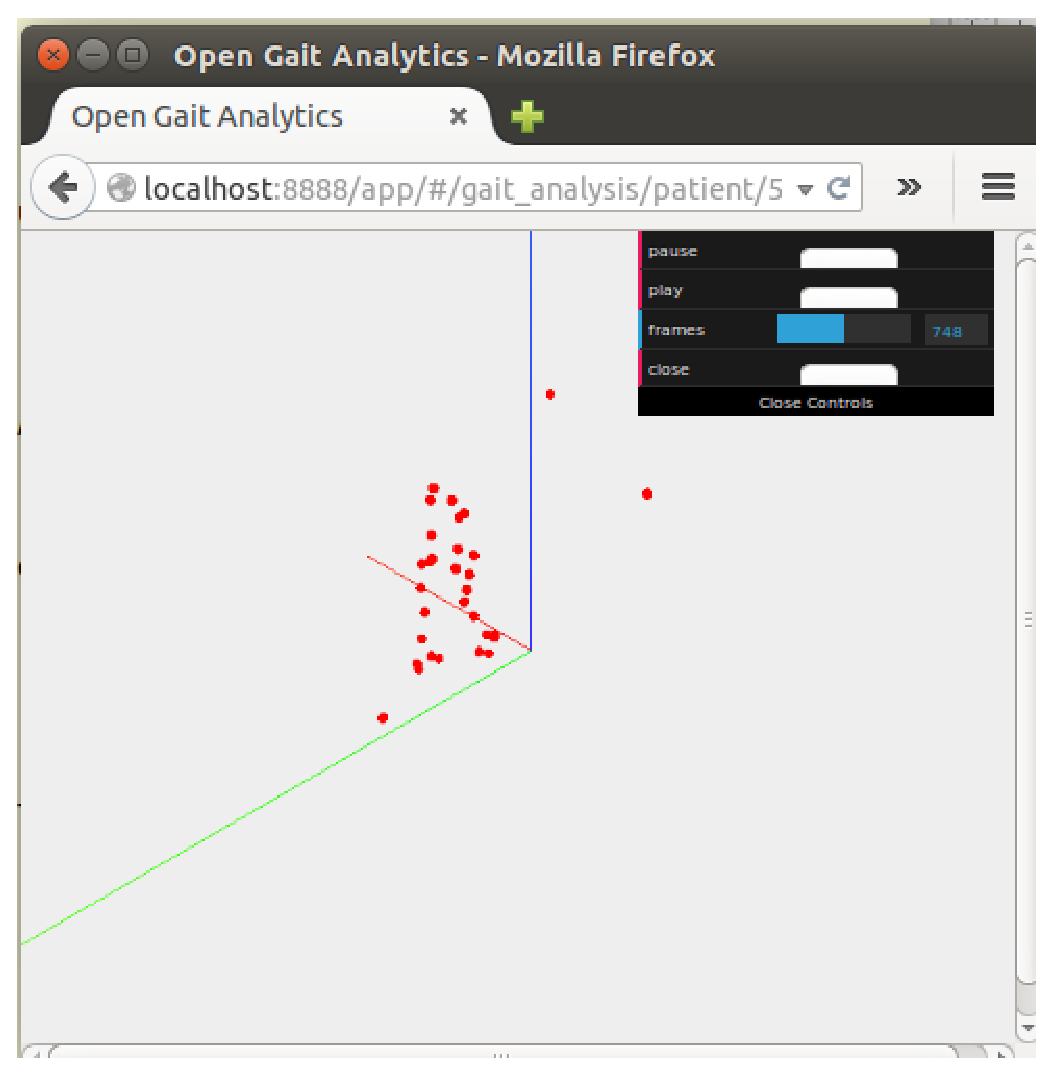
\includegraphics[width=\textwidth]{figuras/tela9.eps}
  \end{minipage}
  \hfill
  \begin{minipage}[b]{0.32\textwidth}
    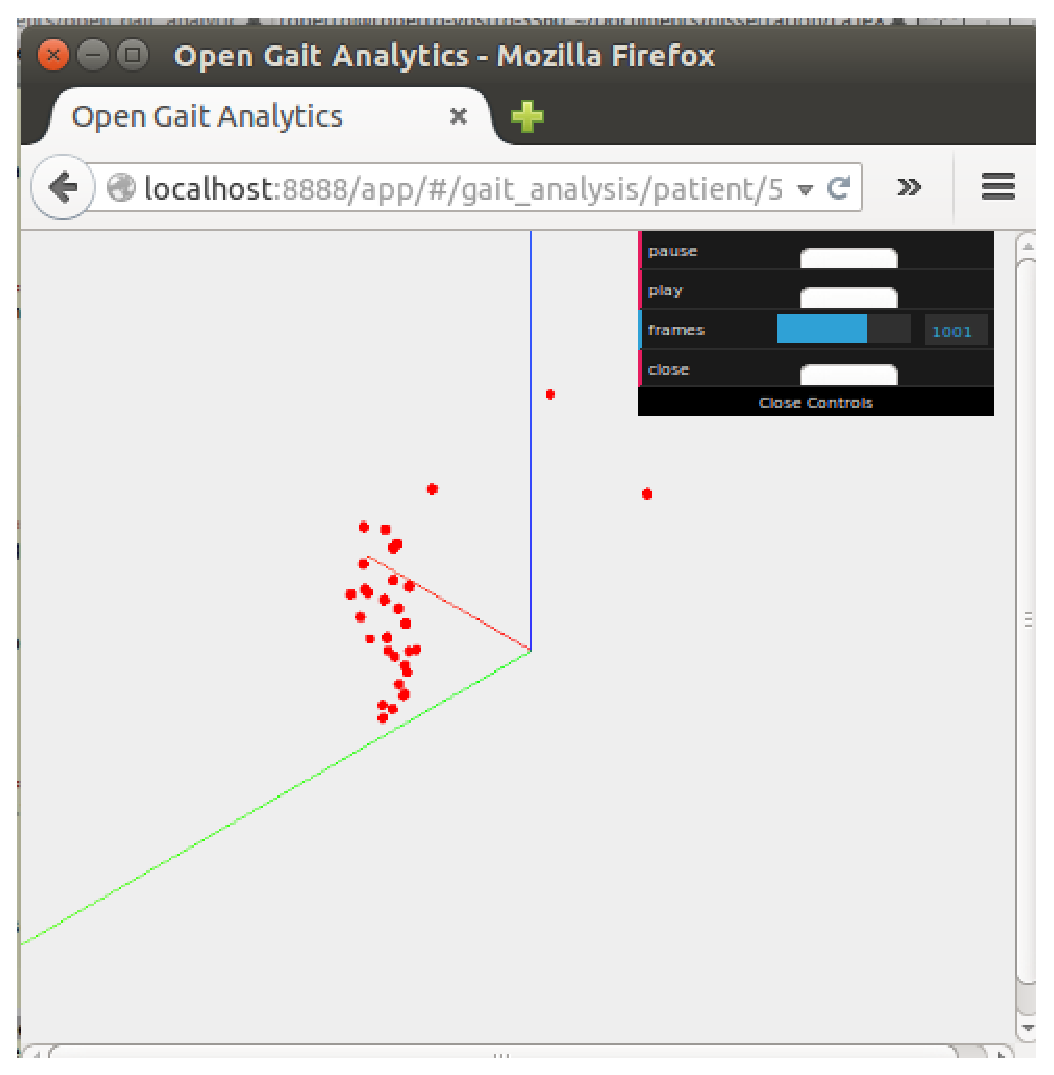
\includegraphics[width=\textwidth]{figuras/tela10.eps}
  \end{minipage}
  \caption[Animação dos marcadores em 3D.]{Animação dos marcadores em 3D. A primeira figura mostra o contato inicial de uma perna. A segunda um momento no período de instância. A terceira o balanço terminal.}
  \label{animacao1}
\end{figure}


A tela da animação também possui controle de perspectivas 
(Figura \ref{animacao2}), controle de \emph{zoom} (Figura \ref{animacao3}), 
e controle \emph{pan} (Figura \ref{animacao4}).
Também foram implementados, até o momento, botões de \emph{play, pause}, fechar e um contador de \emph{frames} (Figura \ref{animacao5}).

\begin{figure}[H]
  \centering
  \begin{minipage}[b]{0.40\textwidth}
    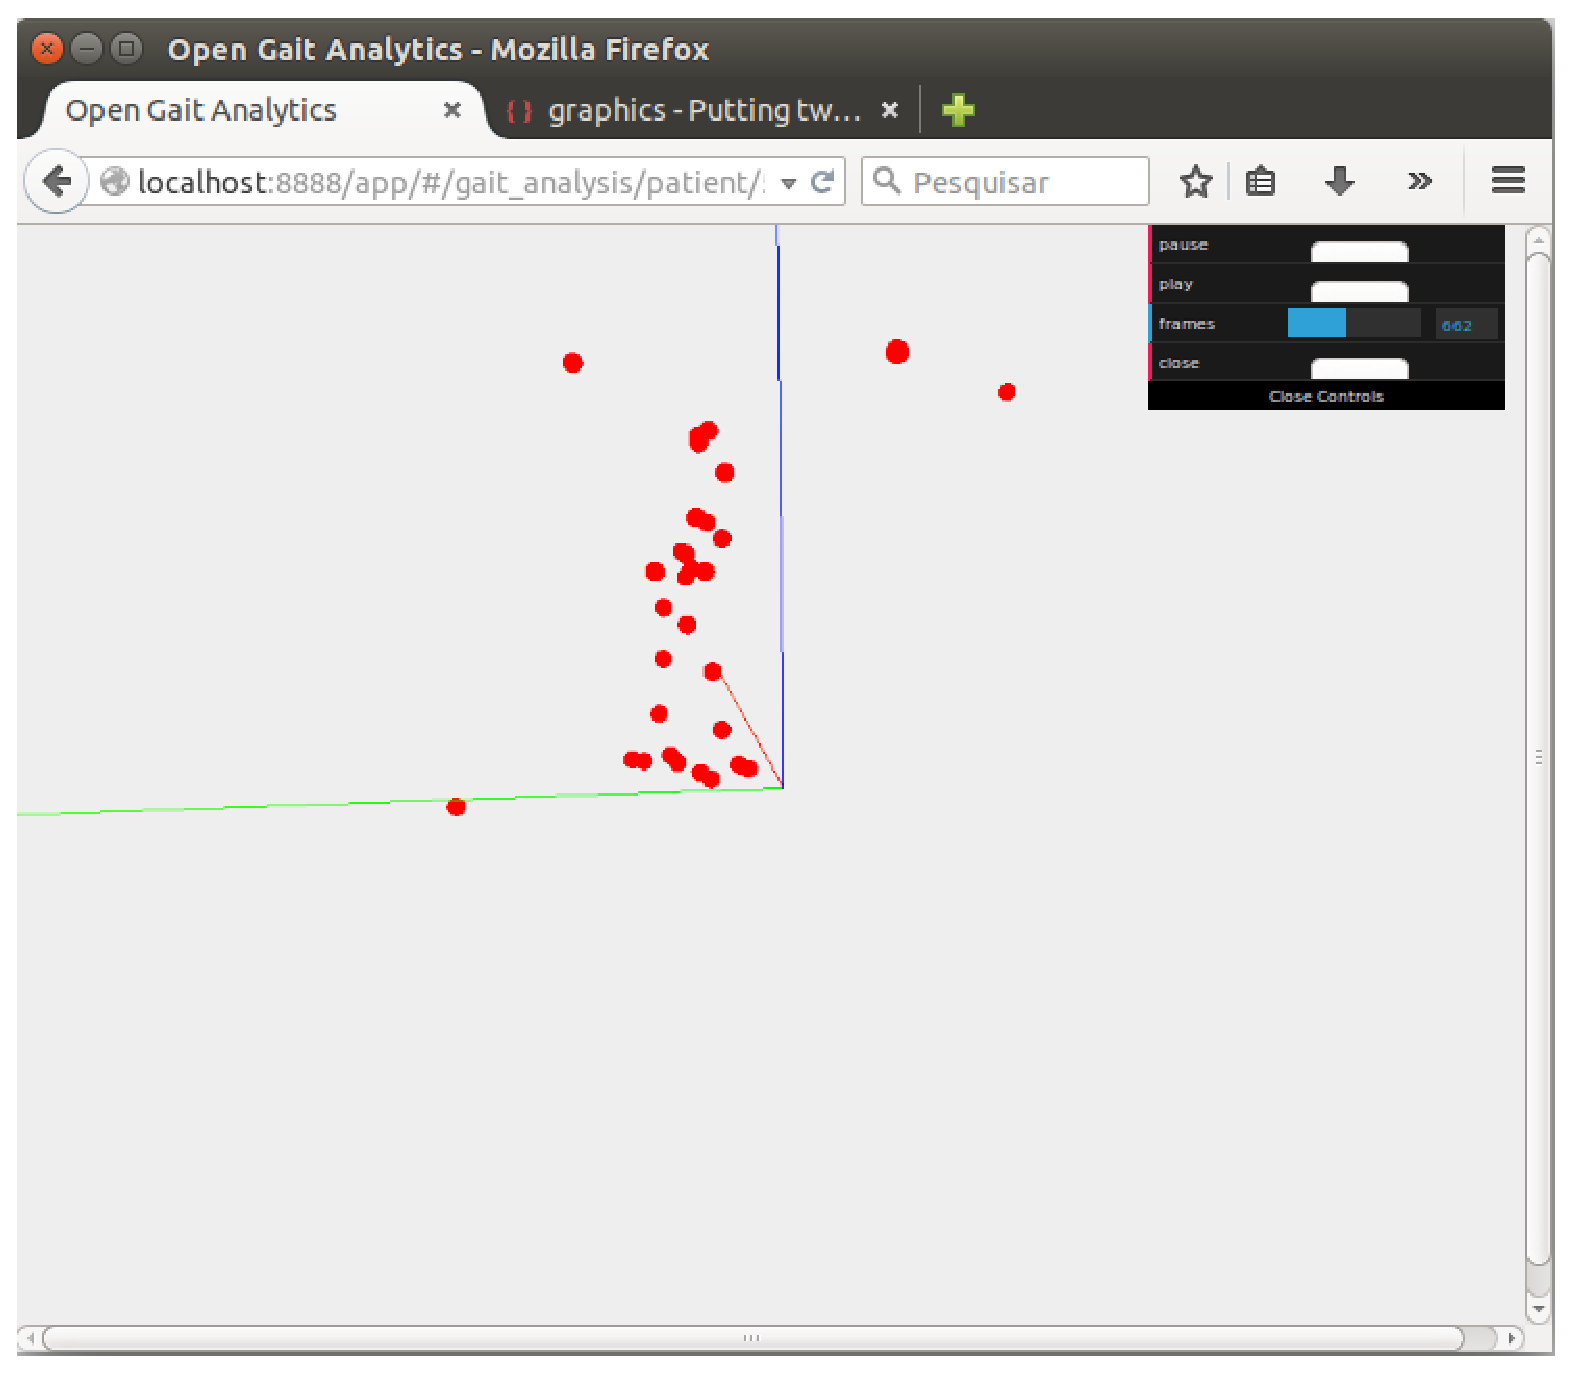
\includegraphics[width=\textwidth]{figuras/tela11.eps}
  \end{minipage}
  \hfill
  \begin{minipage}[b]{0.40\textwidth}
    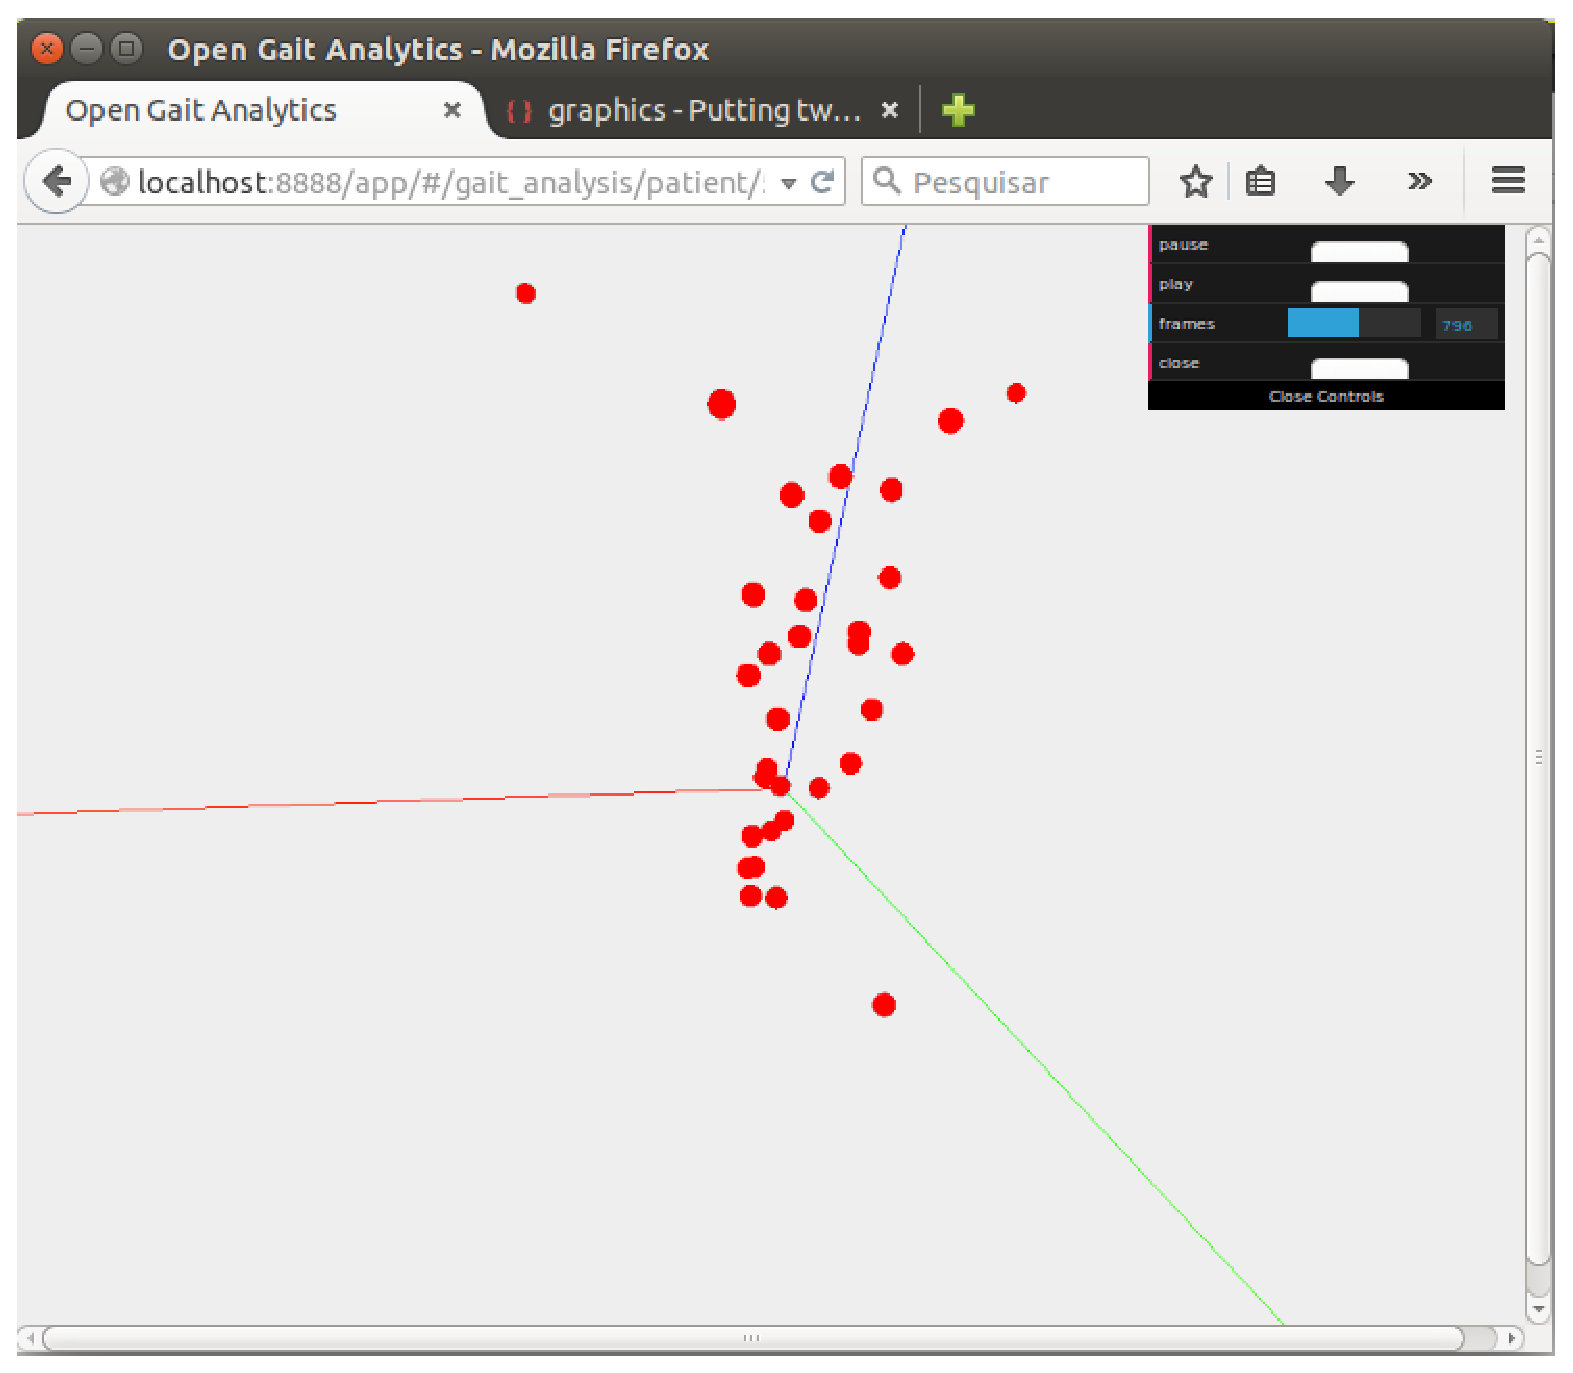
\includegraphics[width=\textwidth]{figuras/tela12.eps}
  \end{minipage}
  \caption[Controle de perspectivas.]{Controle de perspectivas. Primeira figura mostra uma perspectiva lateral do paciente. A segunda figura mostra uma perspectiva diagonal.}
  \label{animacao2}
\end{figure}

\begin{figure}[H]
  \centering
  \begin{minipage}[b]{0.49\textwidth}
    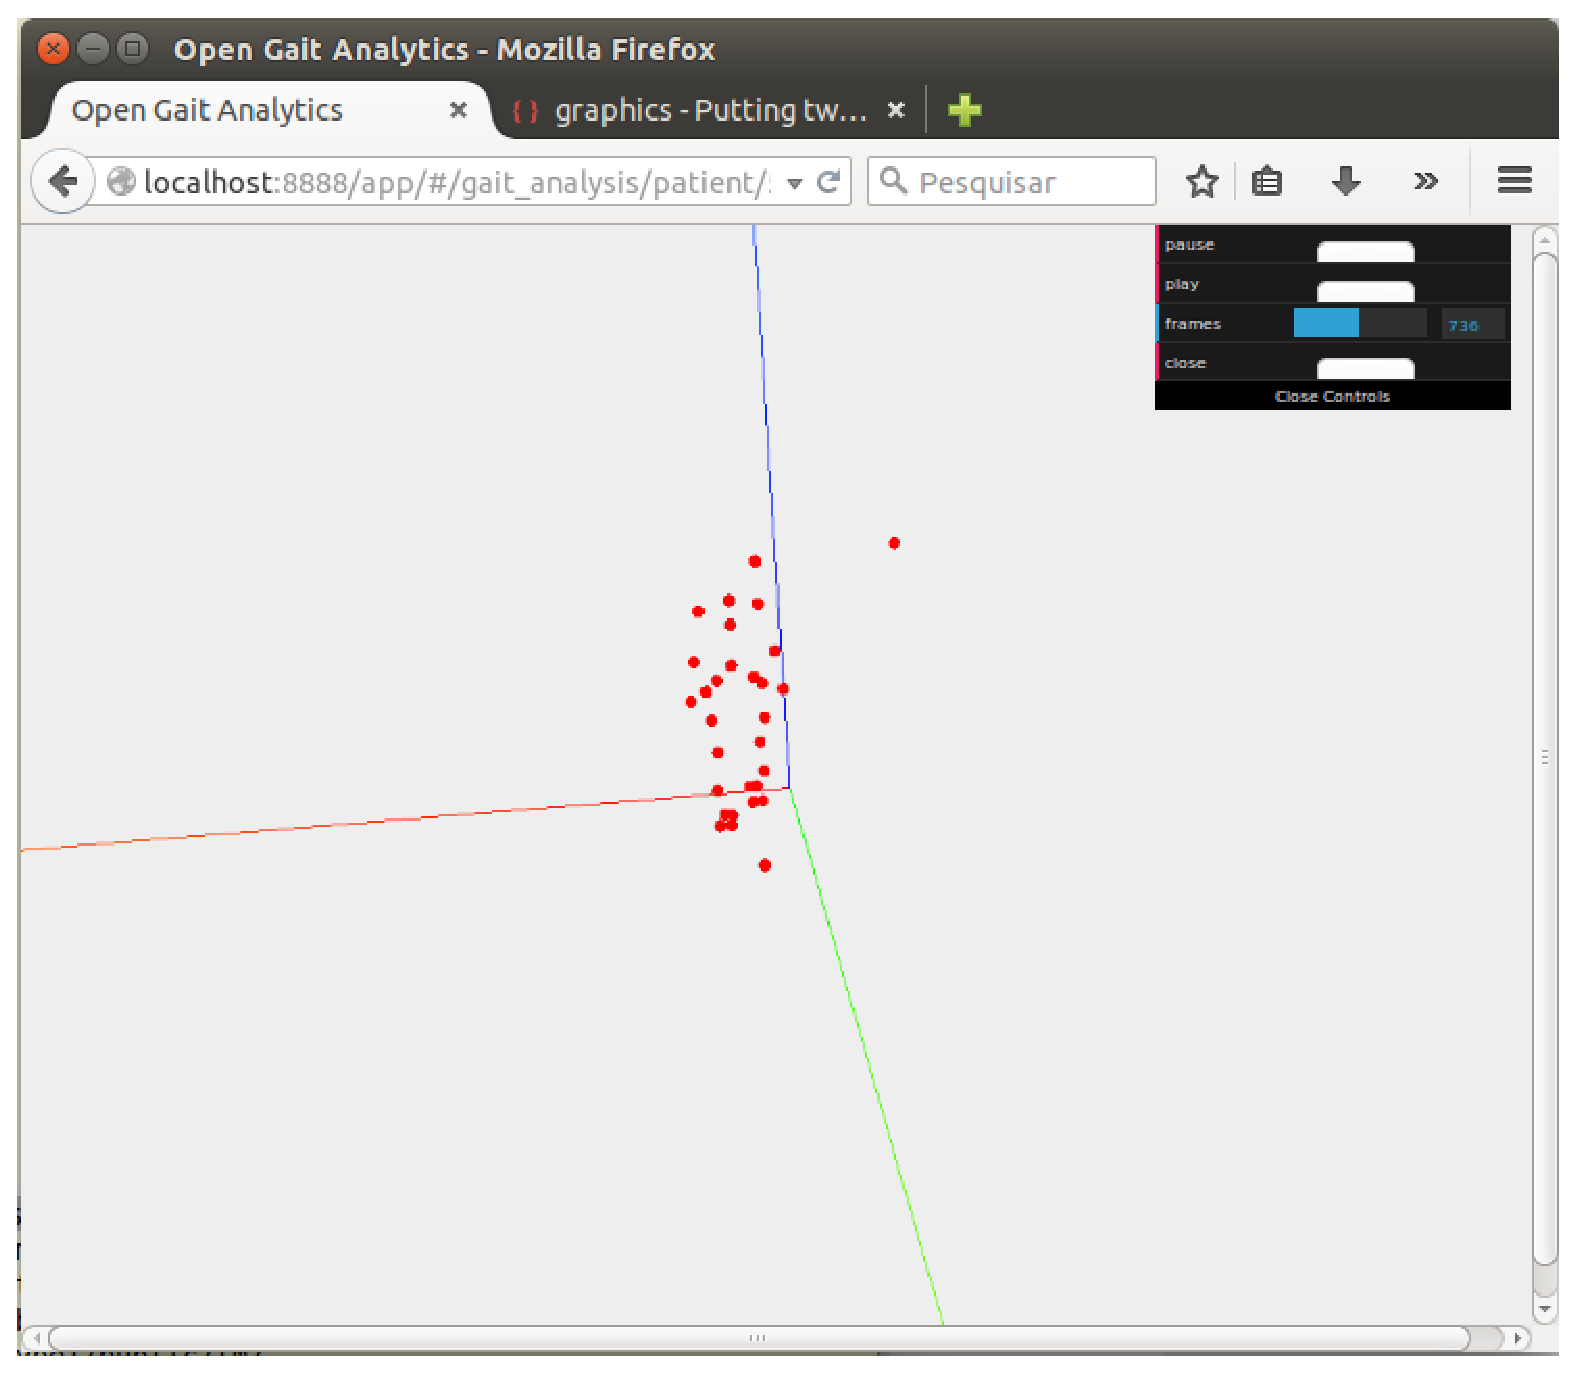
\includegraphics[width=\textwidth]{figuras/tela13.eps}
  \end{minipage}
  \hfill
  \begin{minipage}[b]{0.49\textwidth}
    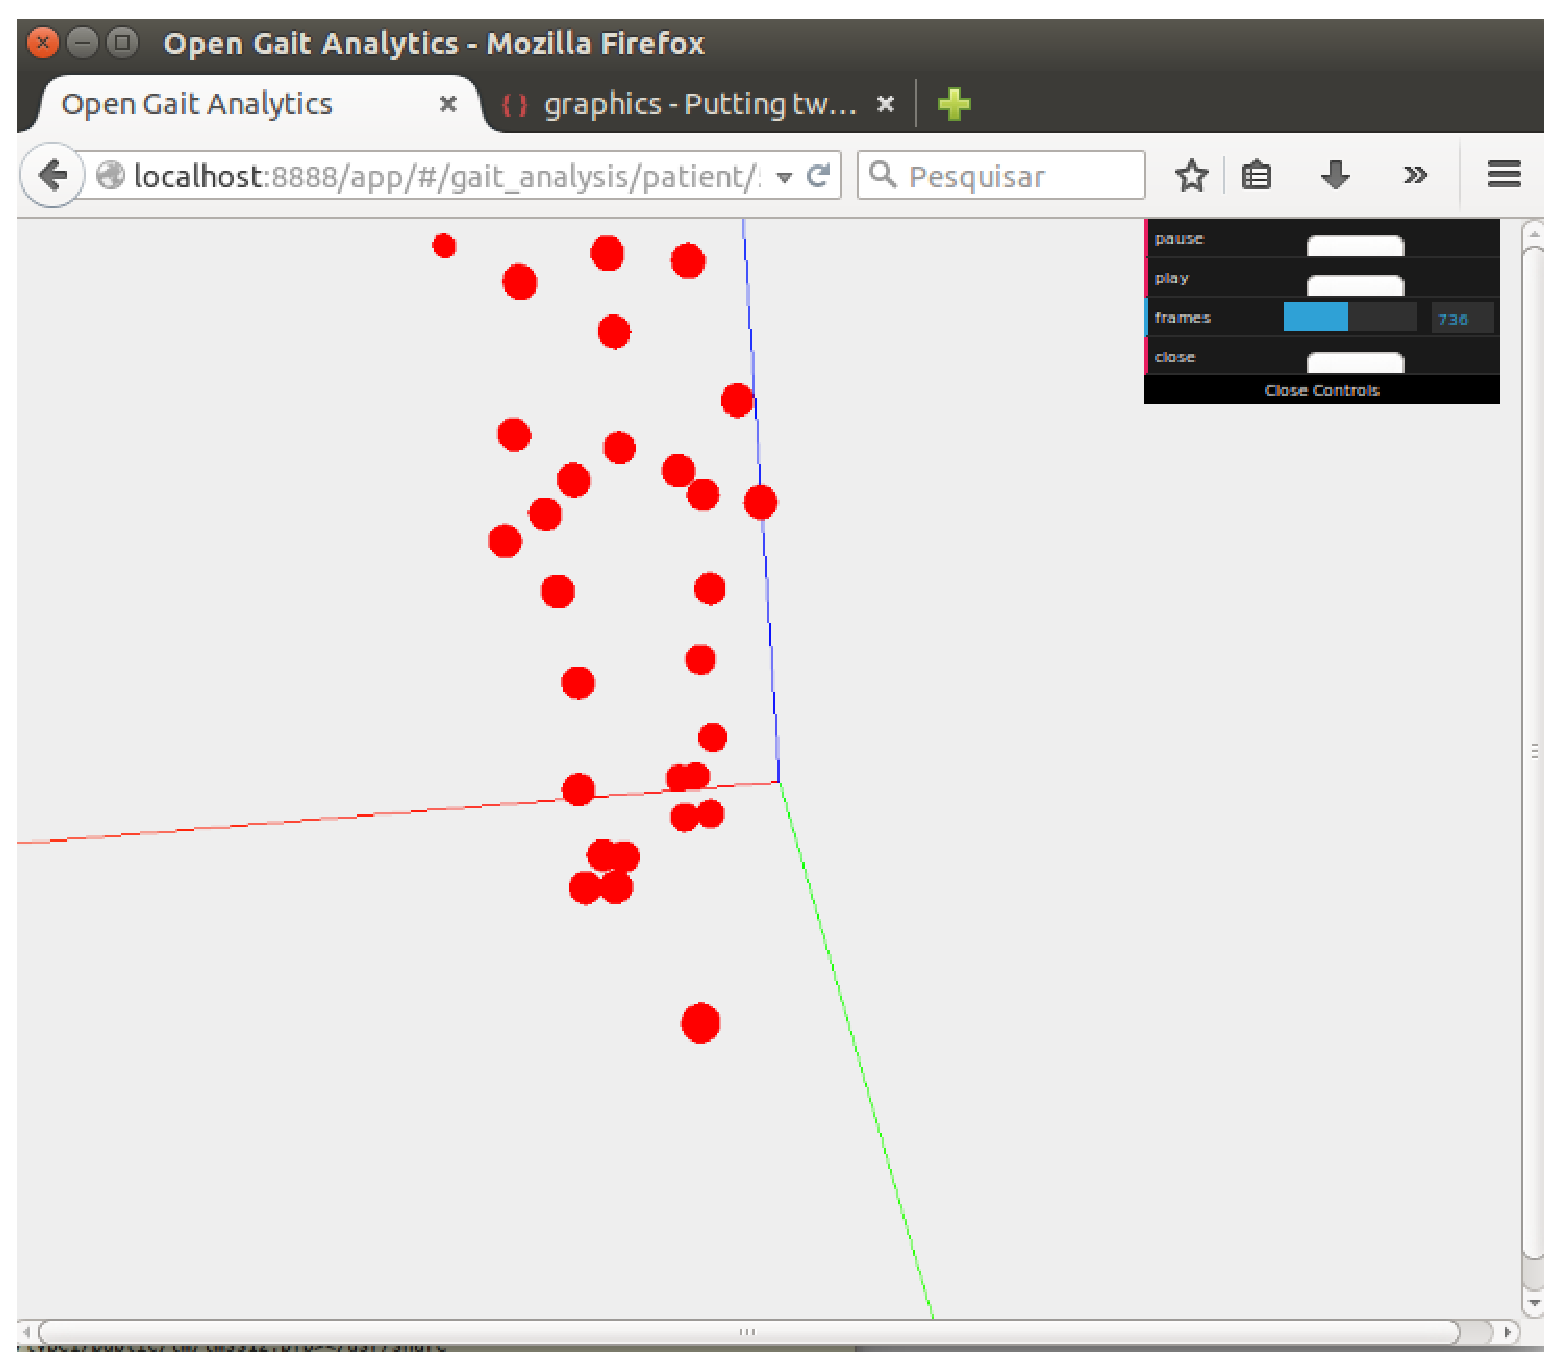
\includegraphics[width=\textwidth]{figuras/tela14.eps}
  \end{minipage}
  \caption[Controle de \emph{zoom}.]{Controle de \emph{zoom}. Primeira figura \emph{zoom out}. Segunda figura \emph{zoom in}.}
  \label{animacao3}
\end{figure}

\begin{figure}[H]
  \centering
  \begin{minipage}[b]{0.49\textwidth}
    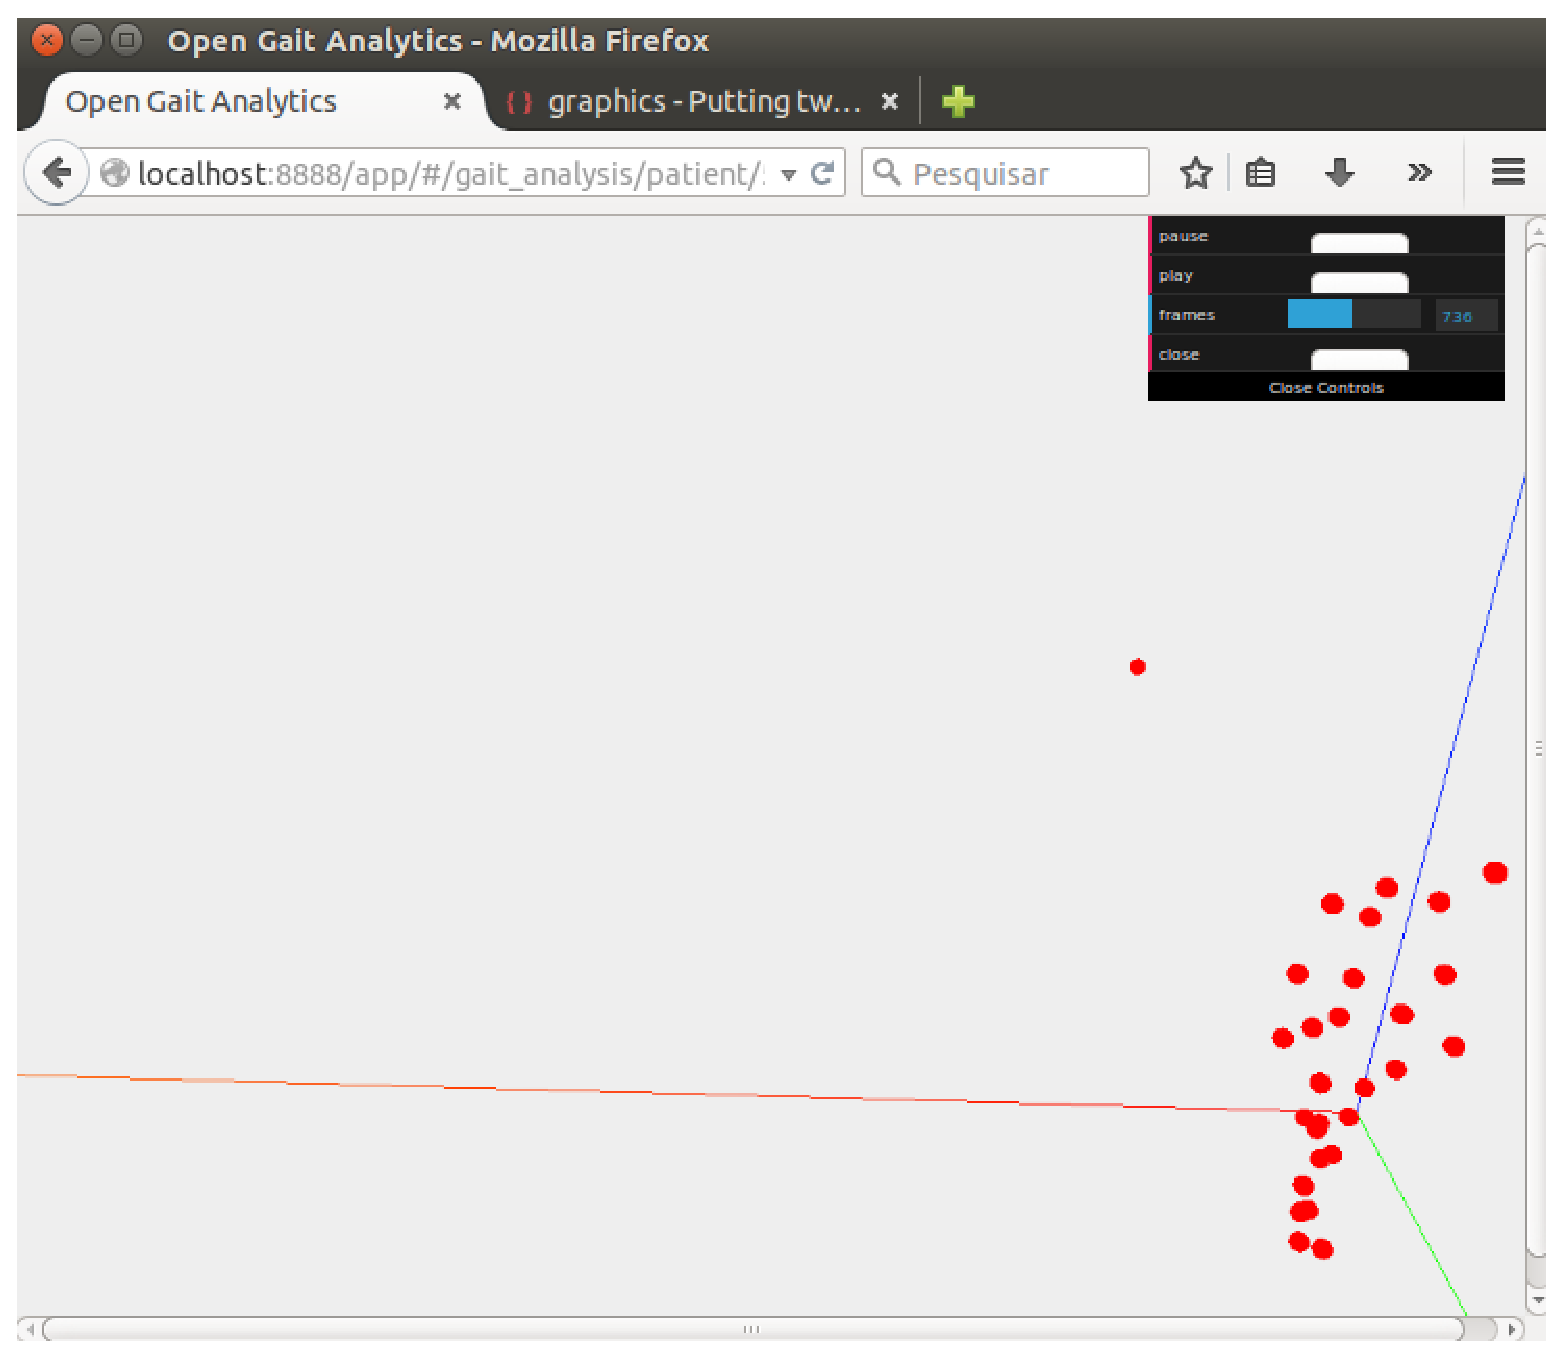
\includegraphics[width=\textwidth]{figuras/tela15.eps}
  \end{minipage}
  \hfill
  \begin{minipage}[b]{0.49\textwidth}
    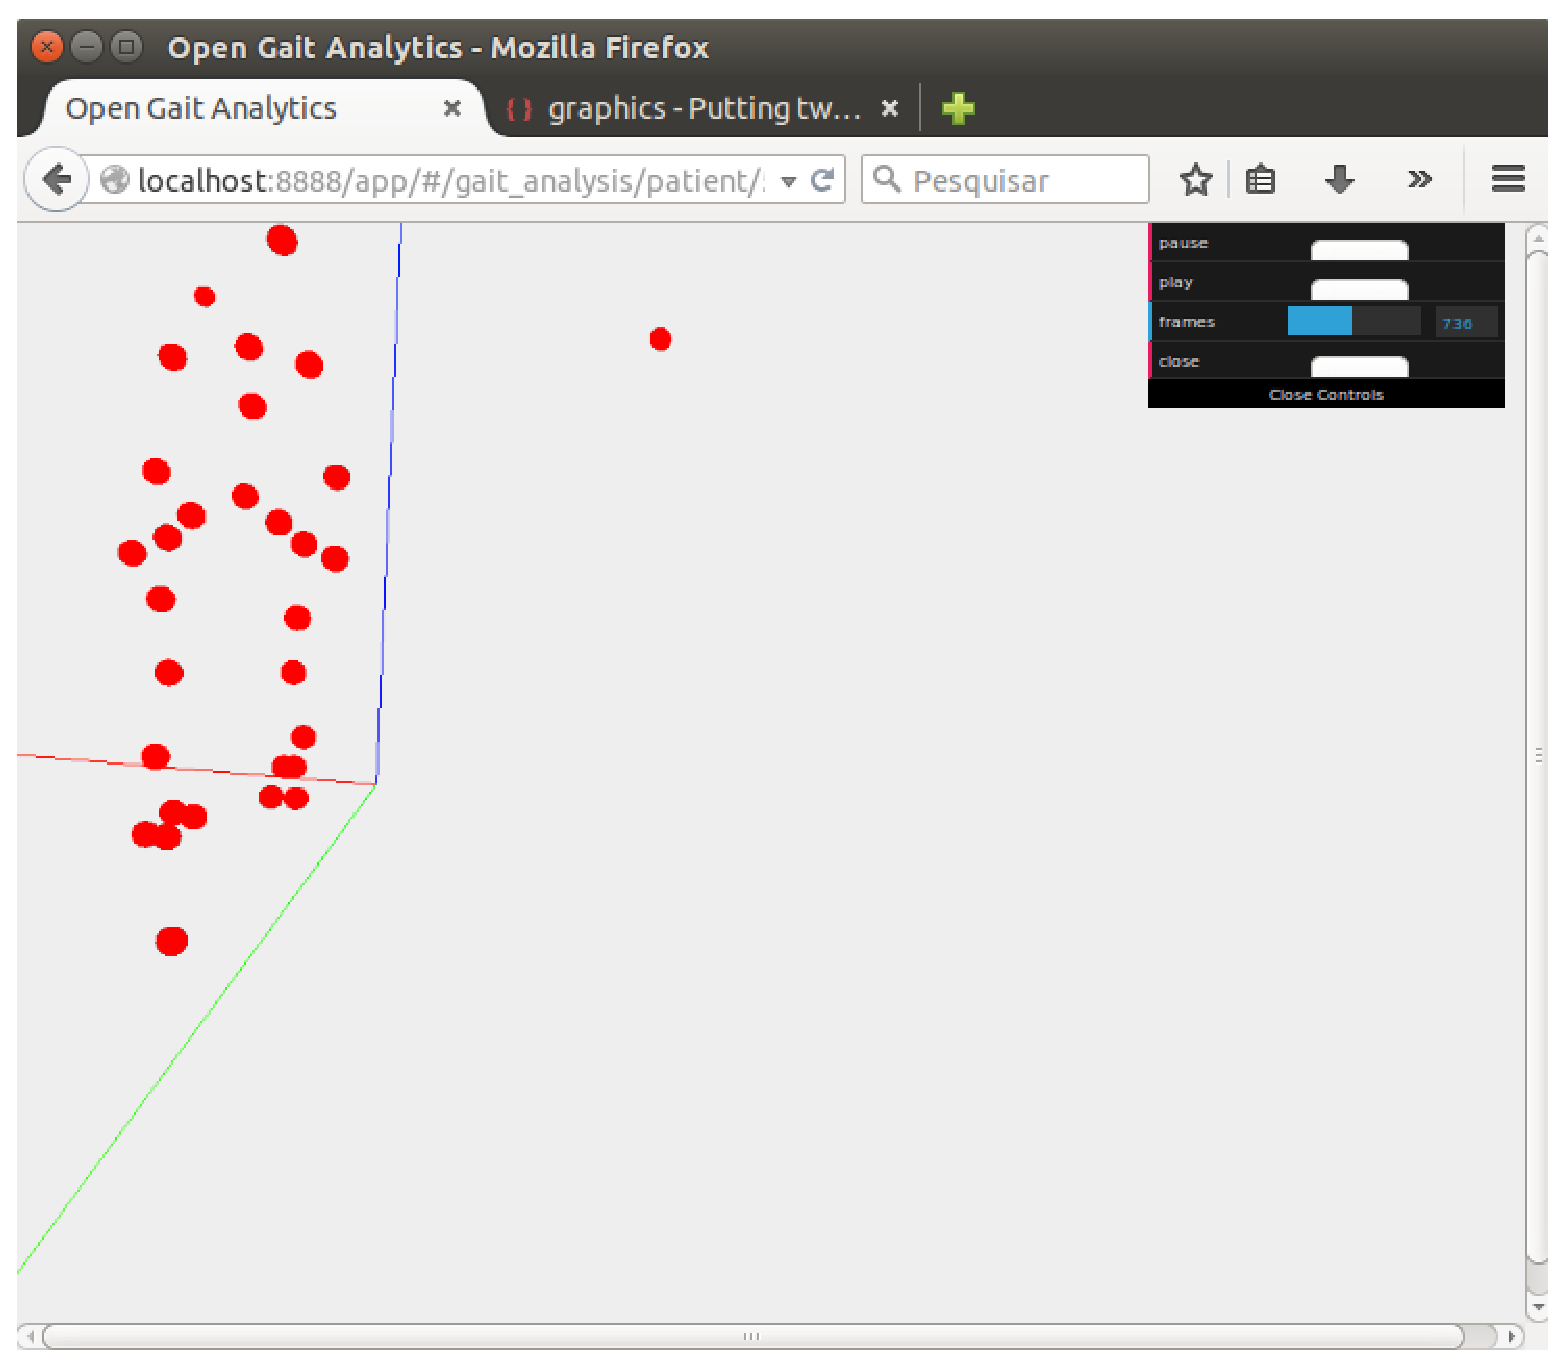
\includegraphics[width=\textwidth]{figuras/tela16.eps}
  \end{minipage}
  \caption[Controle \emph{pan}.]{Controle \emph{pan}. Primeira figura mostra o paciente mais a direita e embaixo. A segunda figura mostra o paciente mais a esquerda e acima.}
  \label{animacao4}
\end{figure}

\begin{figure}[ht]
	\centering
	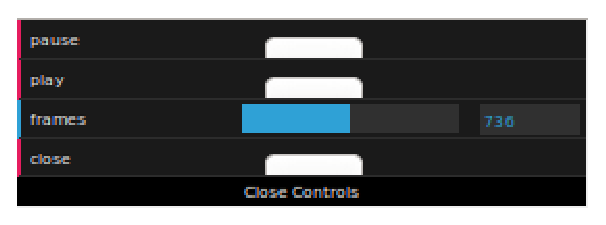
\includegraphics[width=7cm]{figuras/tela17.eps}
	\caption{Controles da animação.}
	\label{animacao5}
\end{figure}






É de fundamental importância que o usuário configure os parâmetros \emph{Initial Contact} e \emph{Terminal Swing} mostrados na Figura \ref{tela7}. Sem estes parâmetros os gráficos, vão mostrar os sinais nas fases erradas do ciclo de marcha.
A técnica que se recomenda é inicializar a animação e quando o usuário perceber o \emph{initial contact}, pressionar o botão \emph{pause} e anotar o \emph{frame}. Fazer a mesma coisa para o \emph{terminal swing}.

Outra opção disponível na Figura \ref{tela7} é a opção \emph{Markers}, esta opção permite nomear os marcadores e visualizar sua progressão espacial. 
A Figura \ref{tela18} mostra o resultado de se selecionar esta opção.
Ao clicar no botão ao lado de algum marcador, sua progressão no espaço é mostrada num gráfico como o da Figura \ref{tela19}. O domínio é o percentual do ciclo de marcha, já a imagem são dados espaciais brutos oriundos do \emph{QTM}.

\begin{figure}[H]
	\centering
	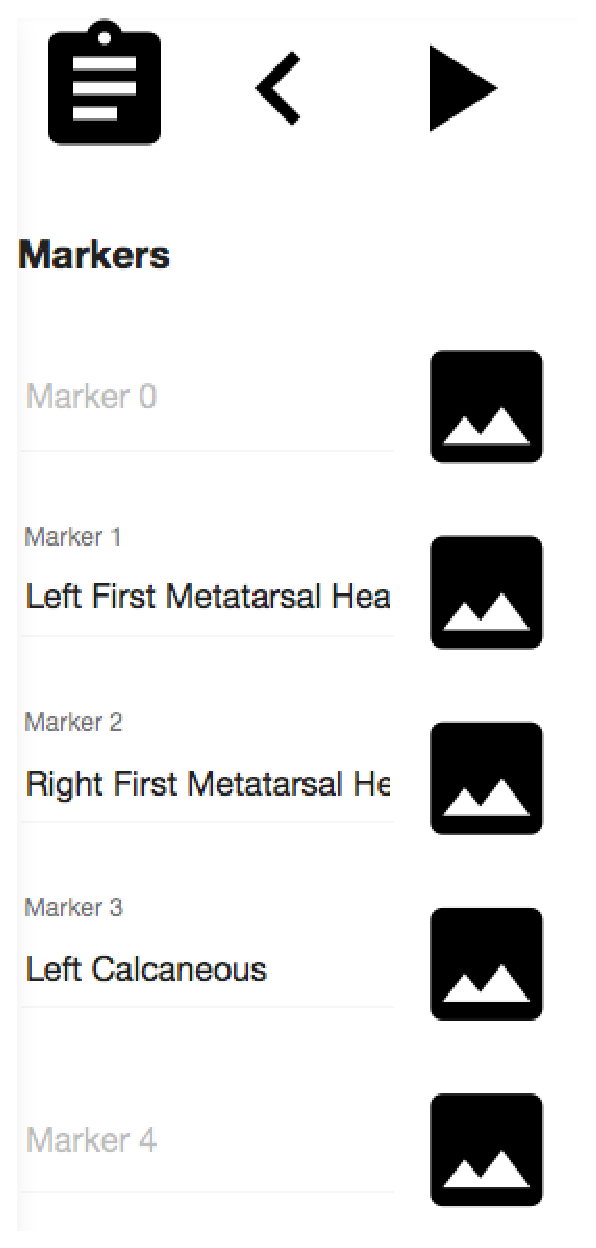
\includegraphics[width=4cm]{figuras/tela18.eps}
	\caption{Opção \emph{markers}.}
	\label{tela18}
\end{figure}


\begin{figure}[H]
	\centering
	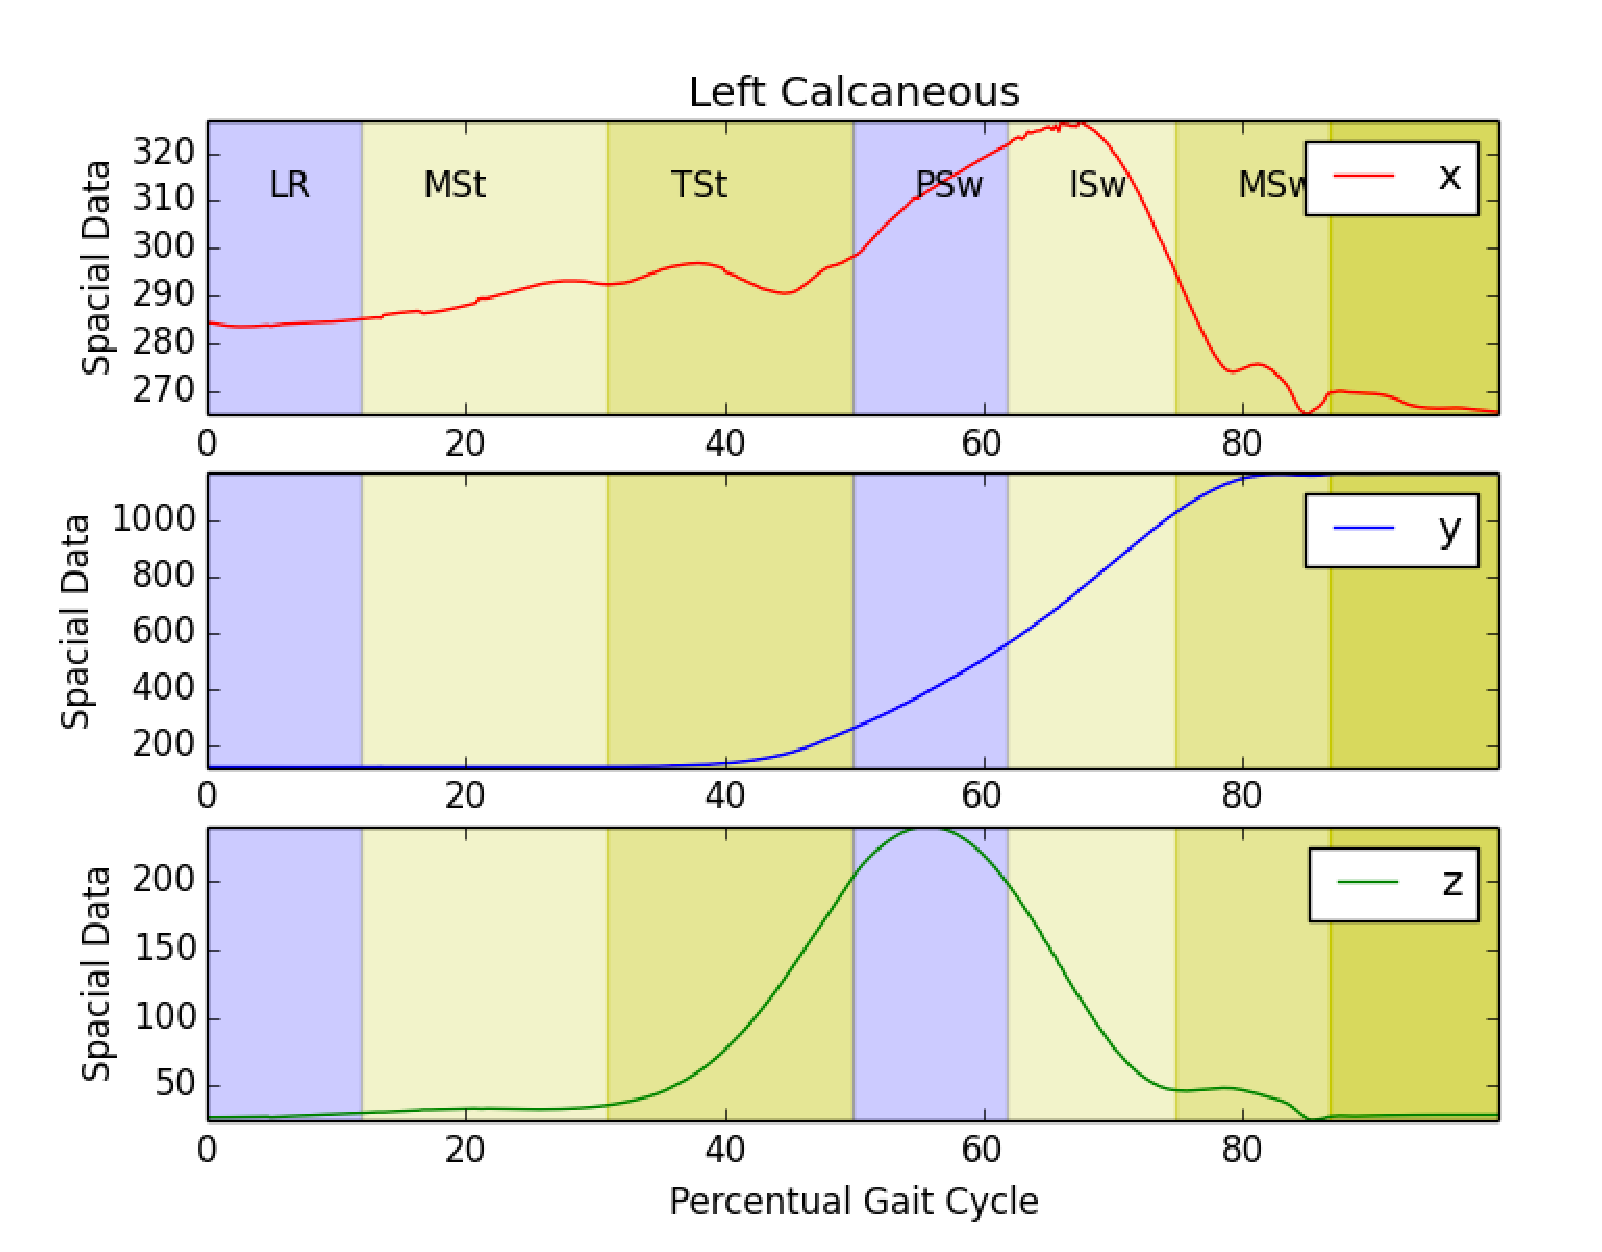
\includegraphics[width=10cm]{figuras/tela19.eps}
	\caption{Progressão espacial de um marcador.}
	\label{tela19}
\end{figure}

A nomeação dos marcadores, não é uma tarefa trivial. Para isso foi criada uma ferramenta dentro da animação para ajudar com esta tarefa. Primeiro, deve-se entrar na animação, depois pausá-la, e posicionar a visualização de uma forma que ajude a detectar o marcador procurado. Veja a Figura \ref{tela20}, nela um marcador foi clicado com o \emph{mouse}, o marcador ficou azul e ao seu lado ele mostra o índice 30. 
Agora é só voltar na opção de marcadores, procurar o índice 30 (\emph{Marker 30}) e colocar o nome desejado. No caso deste marcador o nome é joelho esquerdo (\emph{left knee}, Figura \ref{tela21}).
Agora para o sistema o marcador 30 é sempre o joelho esquerdo (Figura \ref{tela22}).

\begin{figure}[H]
	\centering
	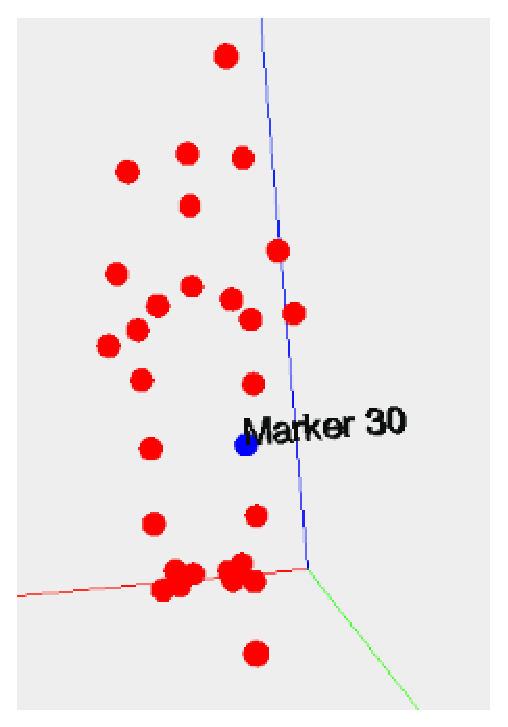
\includegraphics[width=5cm]{figuras/tela20.eps}
	\caption{Seleção de um marcador pelo \emph{mouse}.}
\label{tela20}
\end{figure}

\begin{figure}[H]
	\centering
	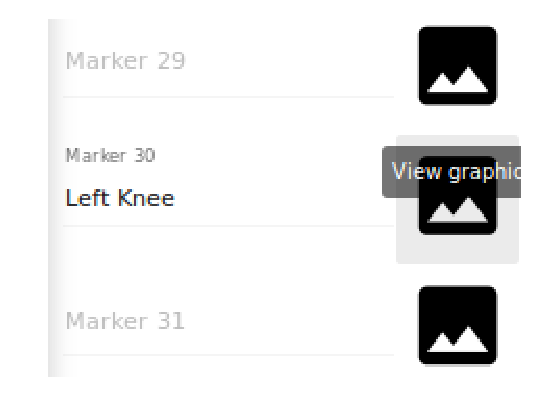
\includegraphics[width=7cm]{figuras/tela21.eps}
	\caption{Renomeando um marcador.}
\label{tela21}
\end{figure}
\begin{figure}[H]
	\centering
	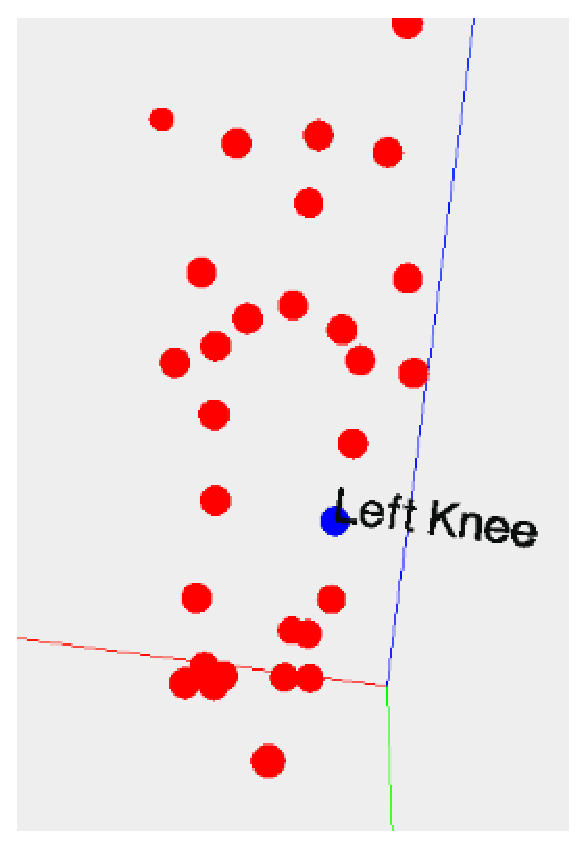
\includegraphics[width=5cm]{figuras/tela22.eps}
	\caption{Animação mostrando o marcador renomeado.}
\label{tela22}

\end{figure}



Outra funcionalidade importante é o gerador de ângulos. Esta opção está disponível na Figura \ref{tela7}. E após selecionada é mostrada na Figura \ref{tela23}. 
Para se gerar um ângulo, o usuário necessita selecionar a opção de inclusão de ângulo e preencher os dados da Figura \ref{tela24}. O usuário precisa indicar a origem do ângulo, por exemplo, o joelho, o componente A, por exemplo, algum músculo da coxa, e o componente B, por exemplo, a tíbia. Estes pontos poderiam representar o ângulo de um joelho, por exemplo.
\begin{figure}[H]
	\centering
	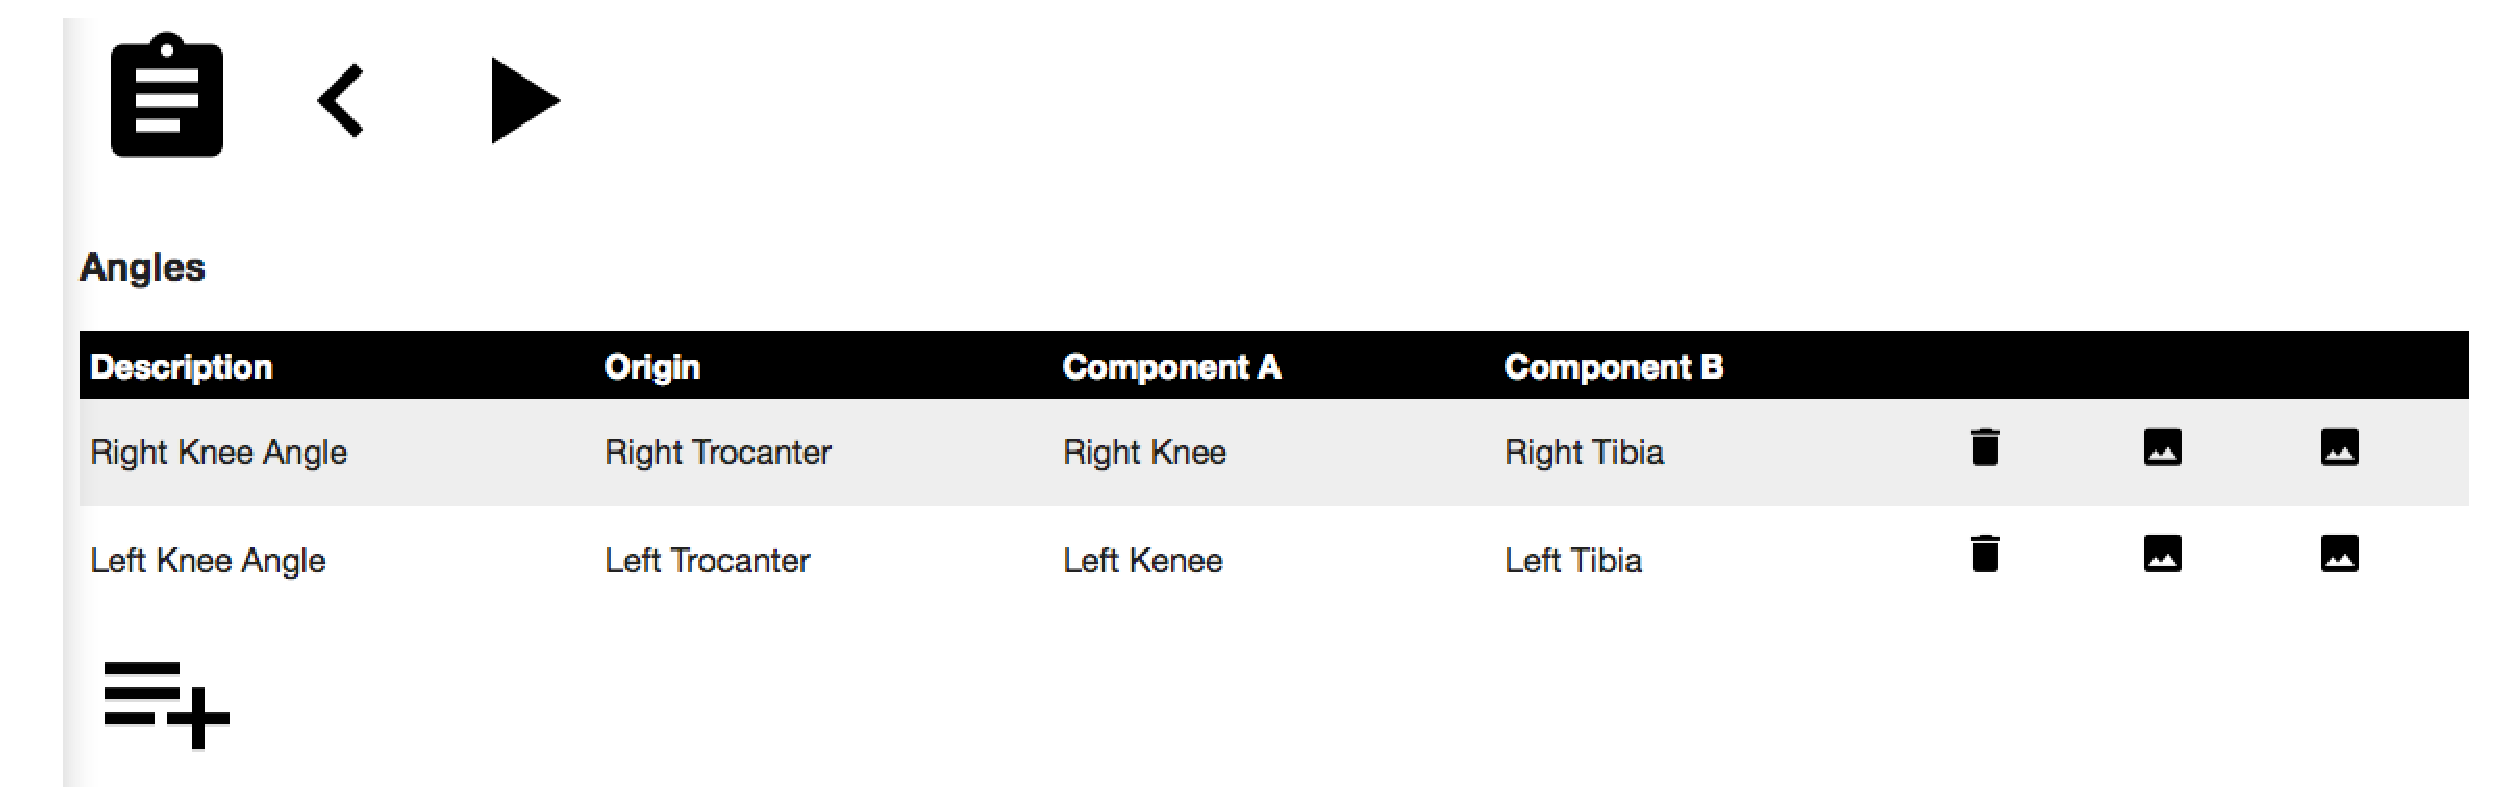
\includegraphics[width=15cm]{figuras/tela23.eps}
	\caption{Opção de visualização e criação de ângulos.}
\label{tela23}
\end{figure}


\begin{figure}[H]
	\centering
	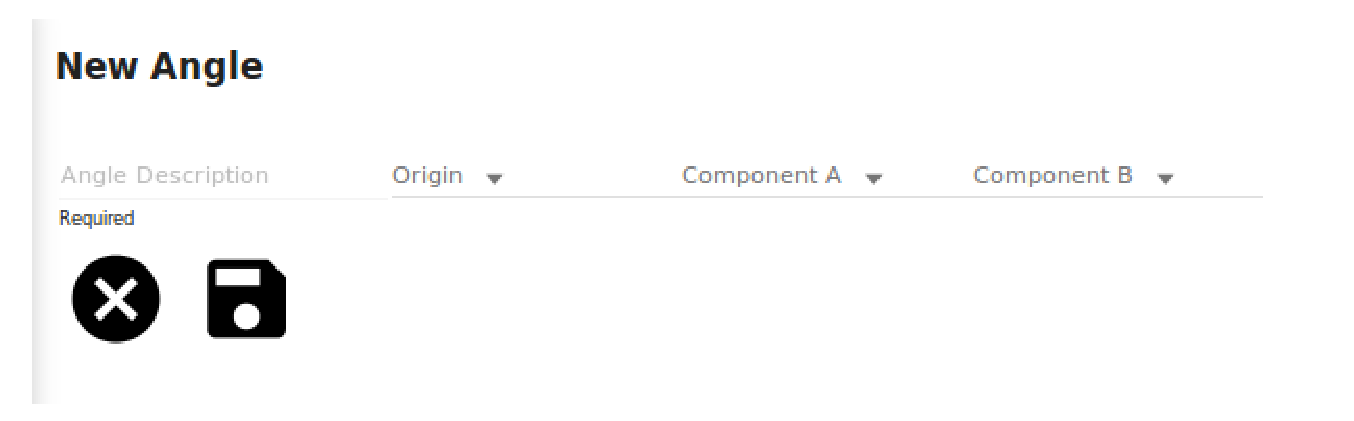
\includegraphics[width=15cm]{figuras/tela24.eps}
	\caption{Inclusão de um novo ângulo.}
\label{tela24}
\end{figure}


Depois dos ângulos criados é possível ver seus valores durante o ciclo de marcha ou suas velocidades angulares, conforme as Figuras \ref{tela25} e \ref{tela26}.
Os ângulos são criados conforme as fórmulas que estão na Seção \ref{cinematica}. O número de pontos usados para o cálculo depende dos parâmetros informados e da quantidade de \emph{frames} por segundo configurada no \emph{QTM}.
\begin{figure}[H]
	\centering
	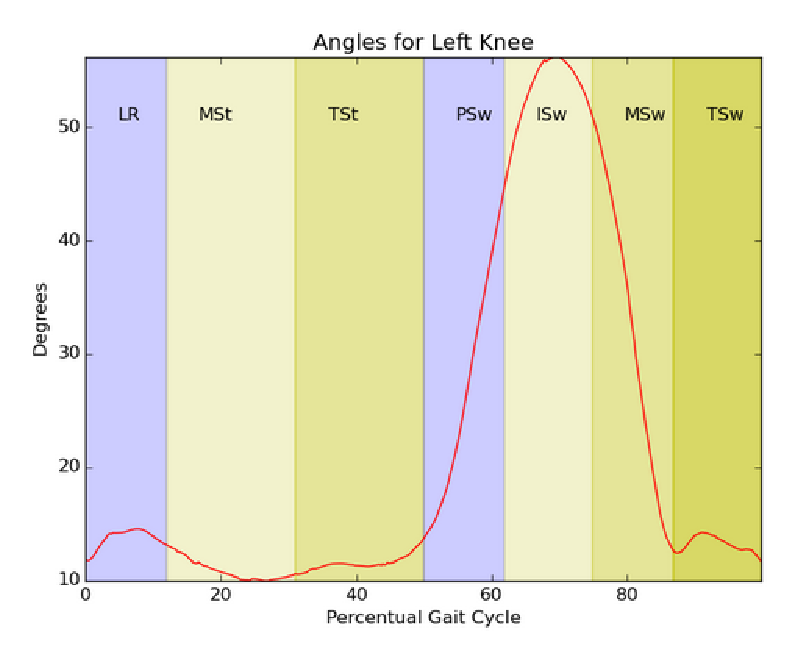
\includegraphics[width=8cm]{figuras/tela25.eps}
	\caption{Ângulo de um joelho durante o ciclo de marcha.}
\label{tela25}
\end{figure}

\begin{figure}[H]
	\centering
	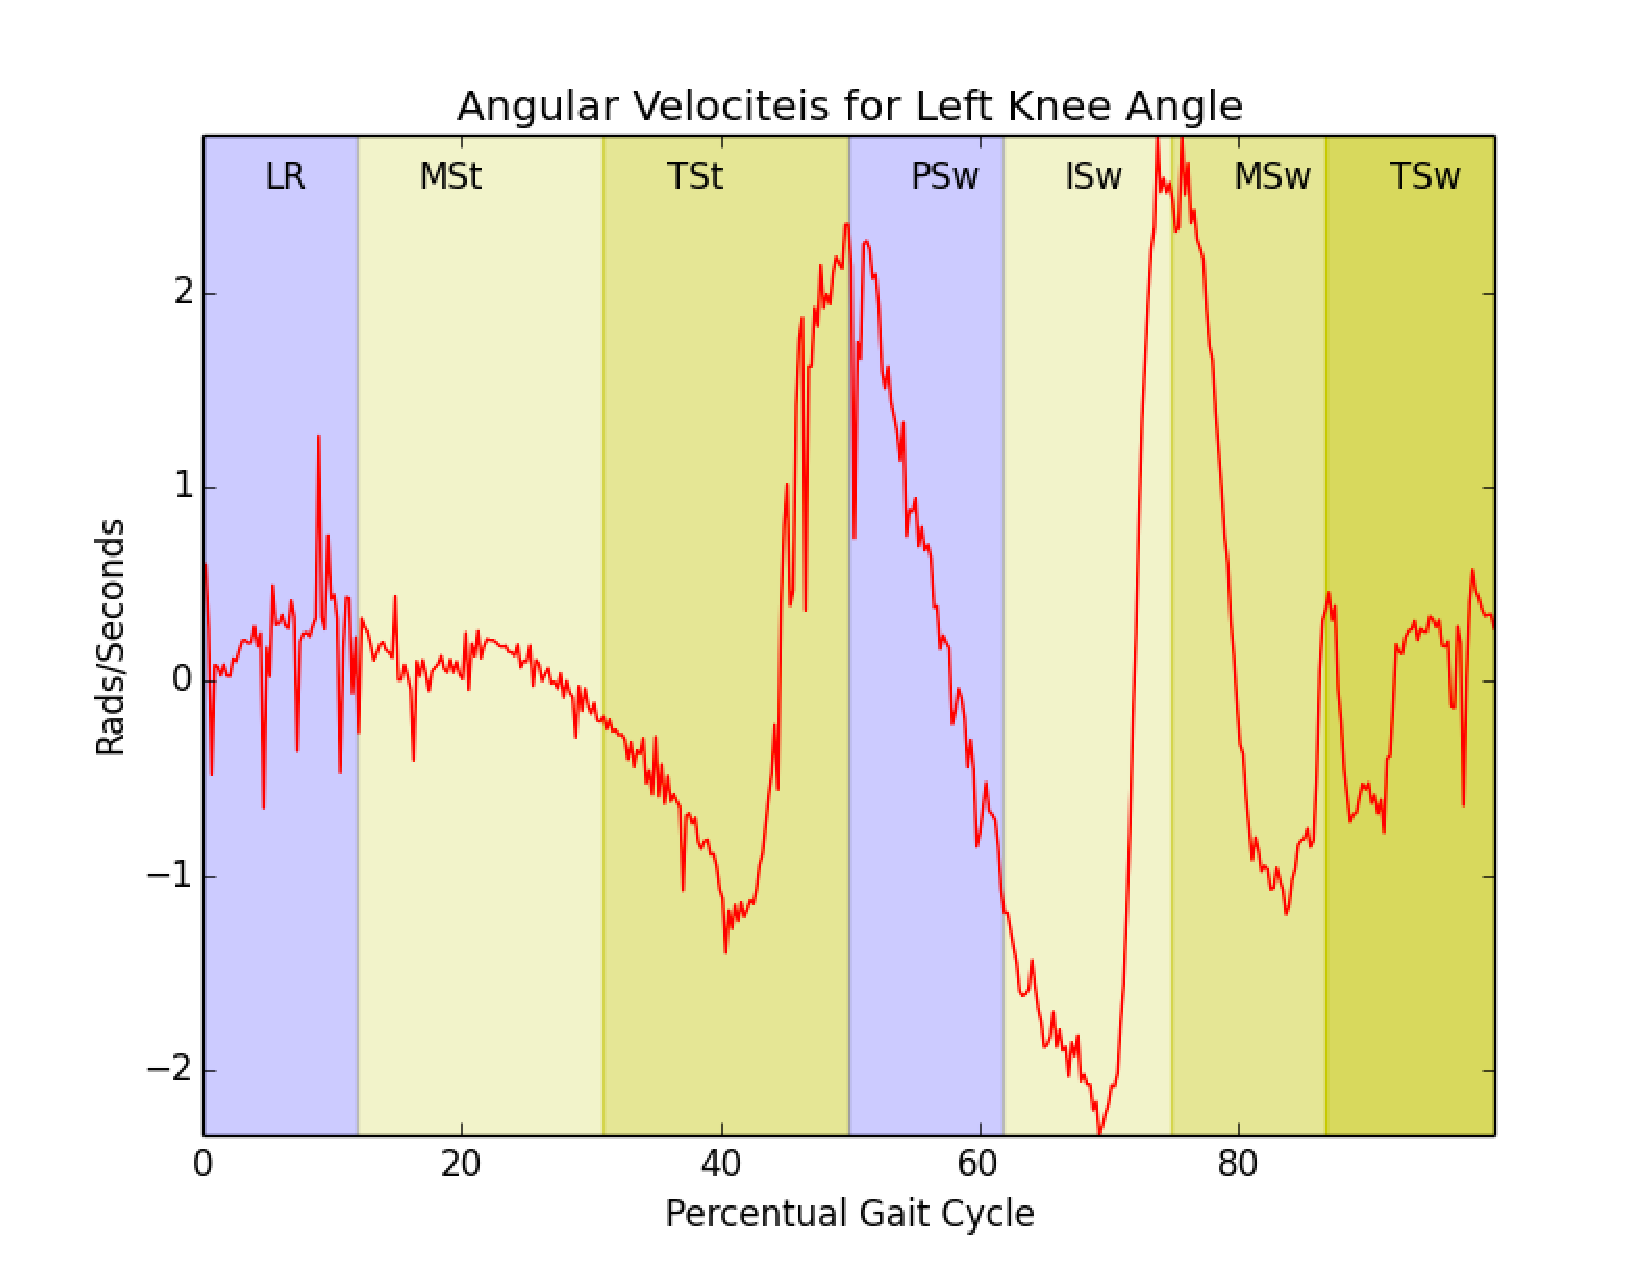
\includegraphics[width=8cm]{figuras/tela26.eps}
	\caption{Velocidades angulares de um joelho durante o ciclo de marcha.}
\label{tela26}
\end{figure}


\section{Módulo de Simulação}
Este módulo é sem dúvida o que mais vai contribuir para os pesquisadores, pois estes contarão com a base integrada gerada pelo módulo de análise e com estas informações será possível realizar simulações de sinais e classificações. 
A versão atual do software ainda é muito pobre neste quesito, mas o objetivo neste momento é mostrar a viabilidade de se usar algoritmos de sistemas inteligentes, integrados na base que vai sendo gerada.
Acredita-se que a ferramenta vai ser mais apreciada por pesquisadores que tem como formação a área de saúde, pois estes não precisarão de todas as técnicas exigidas para fazer simulações num ambiente como o do \emph{MATLAB}.

A primeira funcionalidade de simulação que foi implantada foi a simulação pela \emph{CMAC}, em que esta RNA foi descrita na seção \ref{cmac_sec}. 
Ao se selecionar o módulo simulação, a tela da Figura \ref{tela27} é apresentada. 
A opção \emph{CMAC} já aparece selecionada. 
Para efeitos da demonstração das funcionalidades deste módulo foi realizada uma simulação das velocidades angulares de um joelho, a partir de outros sinais disponíveis.

\begin{figure}[H]
	\centering
	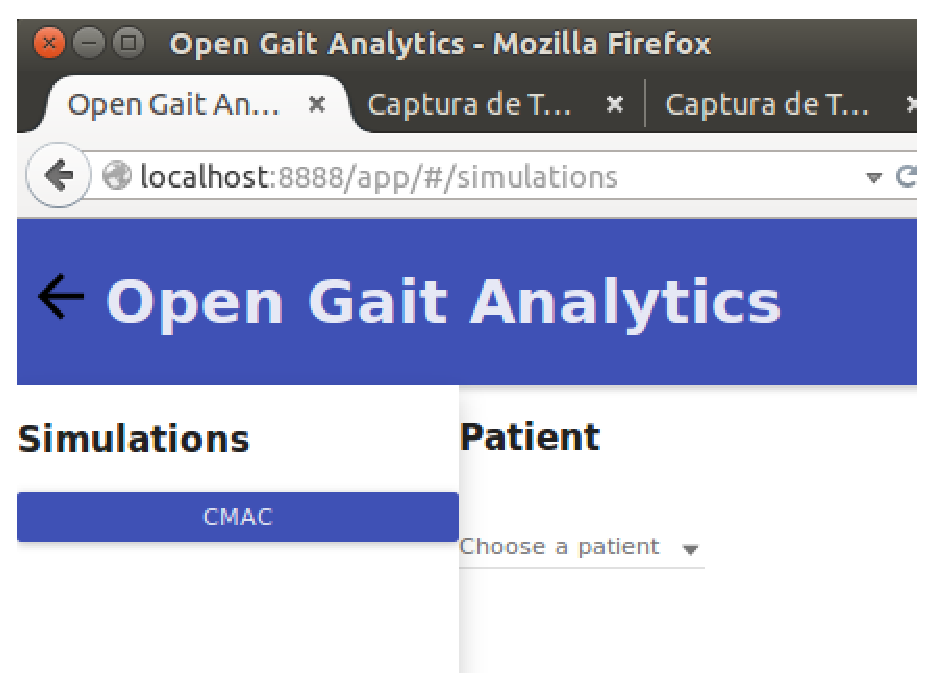
\includegraphics[width=10cm]{figuras/tela27.eps}
	\caption{Módulo de simulação.}
\label{tela27}
\end{figure}


Após ser selecionado o nome de um paciente, deve-se selecionar uma amostra de ciclo de marcha (Figura \ref{tela28}).
Após a seleção do ciclo de marcha, uma lista com vários sinais são mostrados, basicamente os sinais são coordenadas de posições de marcadores, ângulos e velocidades angulares. As Figuras \ref{tela29} e \ref{tela30} mostram uma fração dos sinais possíveis para seleção. Ao se selecionar um sinal de entrada é necessário também informar sua quantização.
\begin{figure}[H]
	\centering
	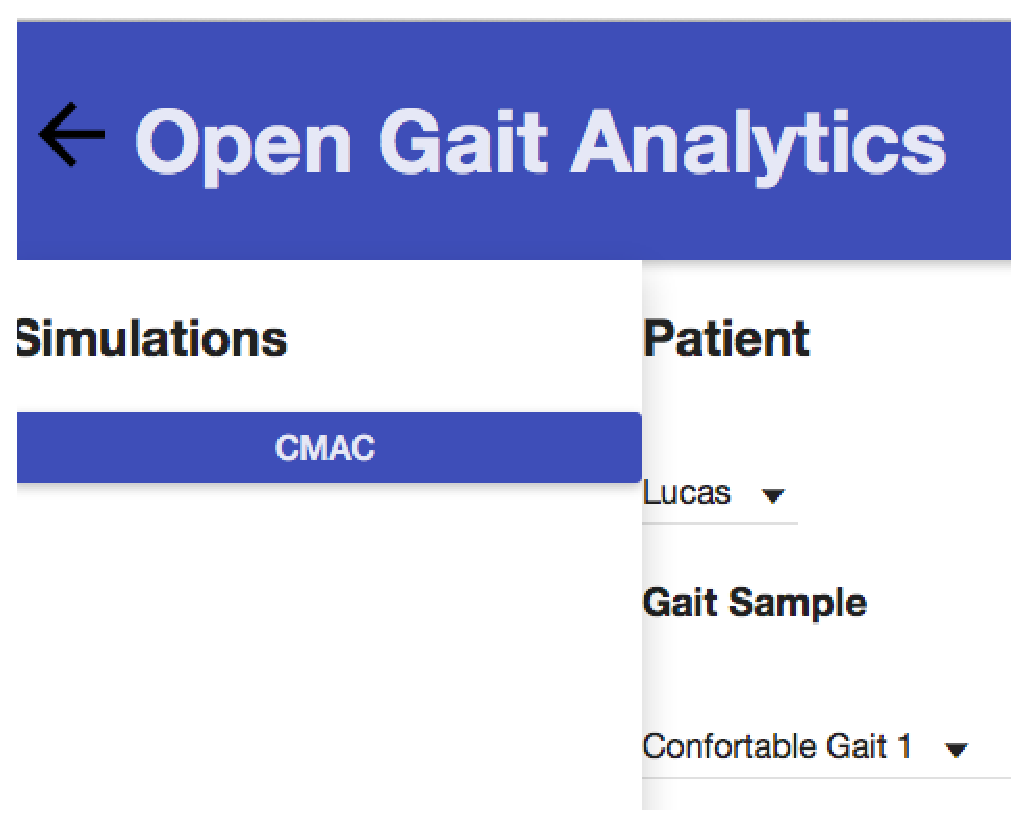
\includegraphics[width=10cm]{figuras/tela28.eps}
	\caption{Seleção do ciclo de marcha.}
\label{tela28}
\end{figure}

\begin{figure}[H]
	\centering
	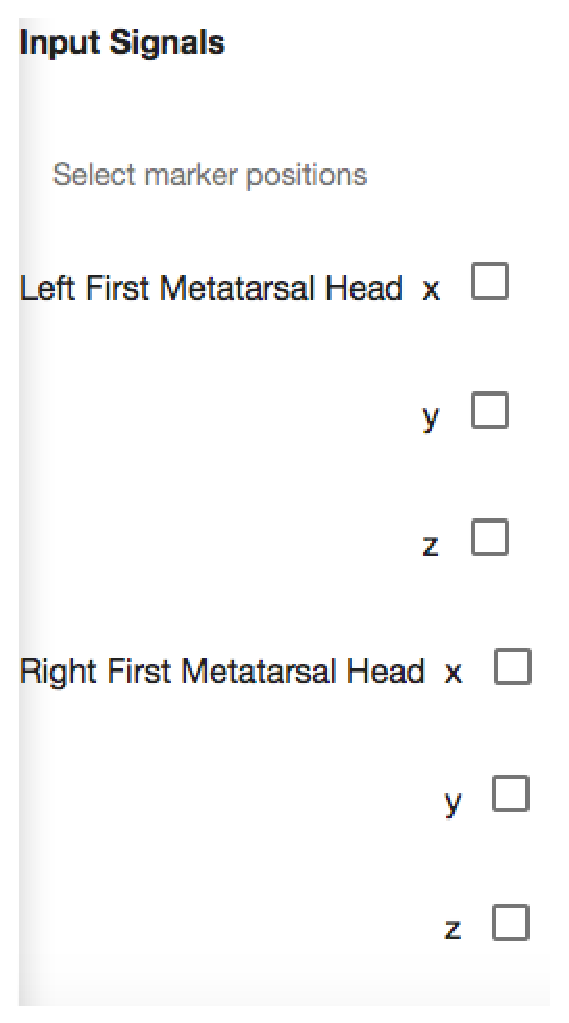
\includegraphics[width=5cm]{figuras/tela29.eps}
	\caption{Sinais de entrada para a \emph{CMAC}. No caso posições num plano 3D de marcadores.}
\label{tela29}
\end{figure}

\begin{figure}[H]
	\centering
	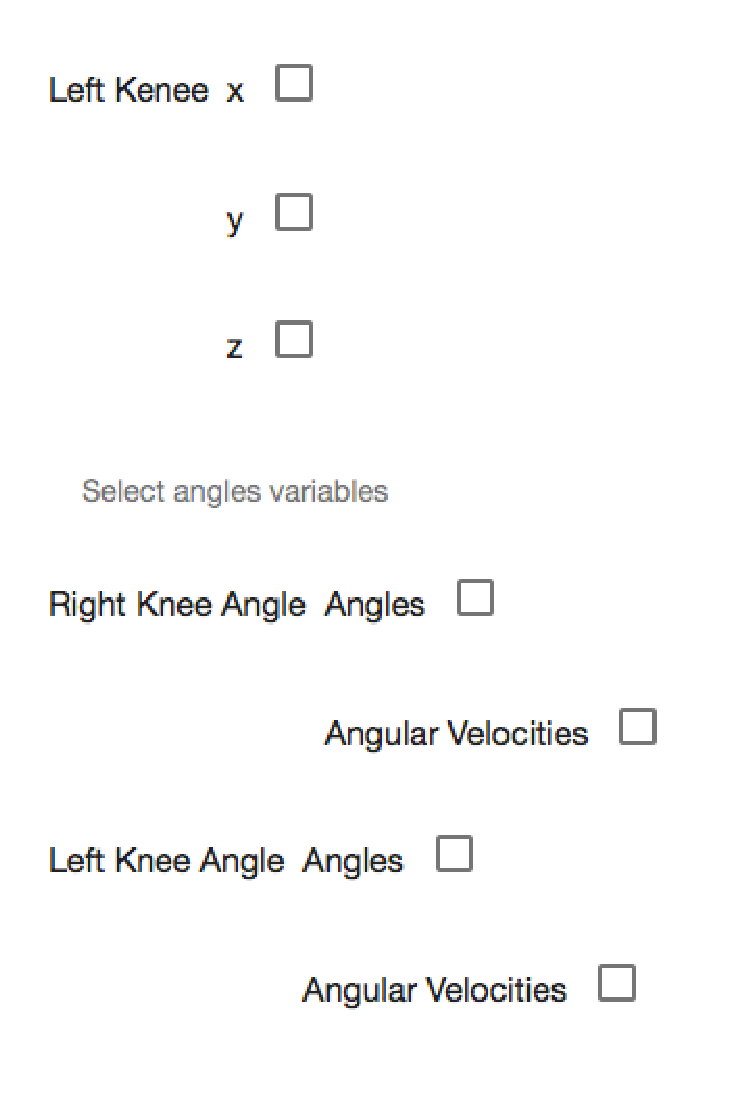
\includegraphics[width=5cm]{figuras/tela30.eps}
	\caption{Sinais de entrada para a \emph{CMAC}, ângulos e velocidades angulares.}
\label{tela30}
\end{figure}


A Figura \ref{tela31} mostra uma configuração que gera a saída da Figura \ref{tela32}.  O gráfico mostrado é a saída da RNA  \emph{CMAC}. 
A Figura \ref{tela33} mostra o erro quadrado médio da execução da simulação ao longo das iterações.
\begin{figure}[H]
	\centering
	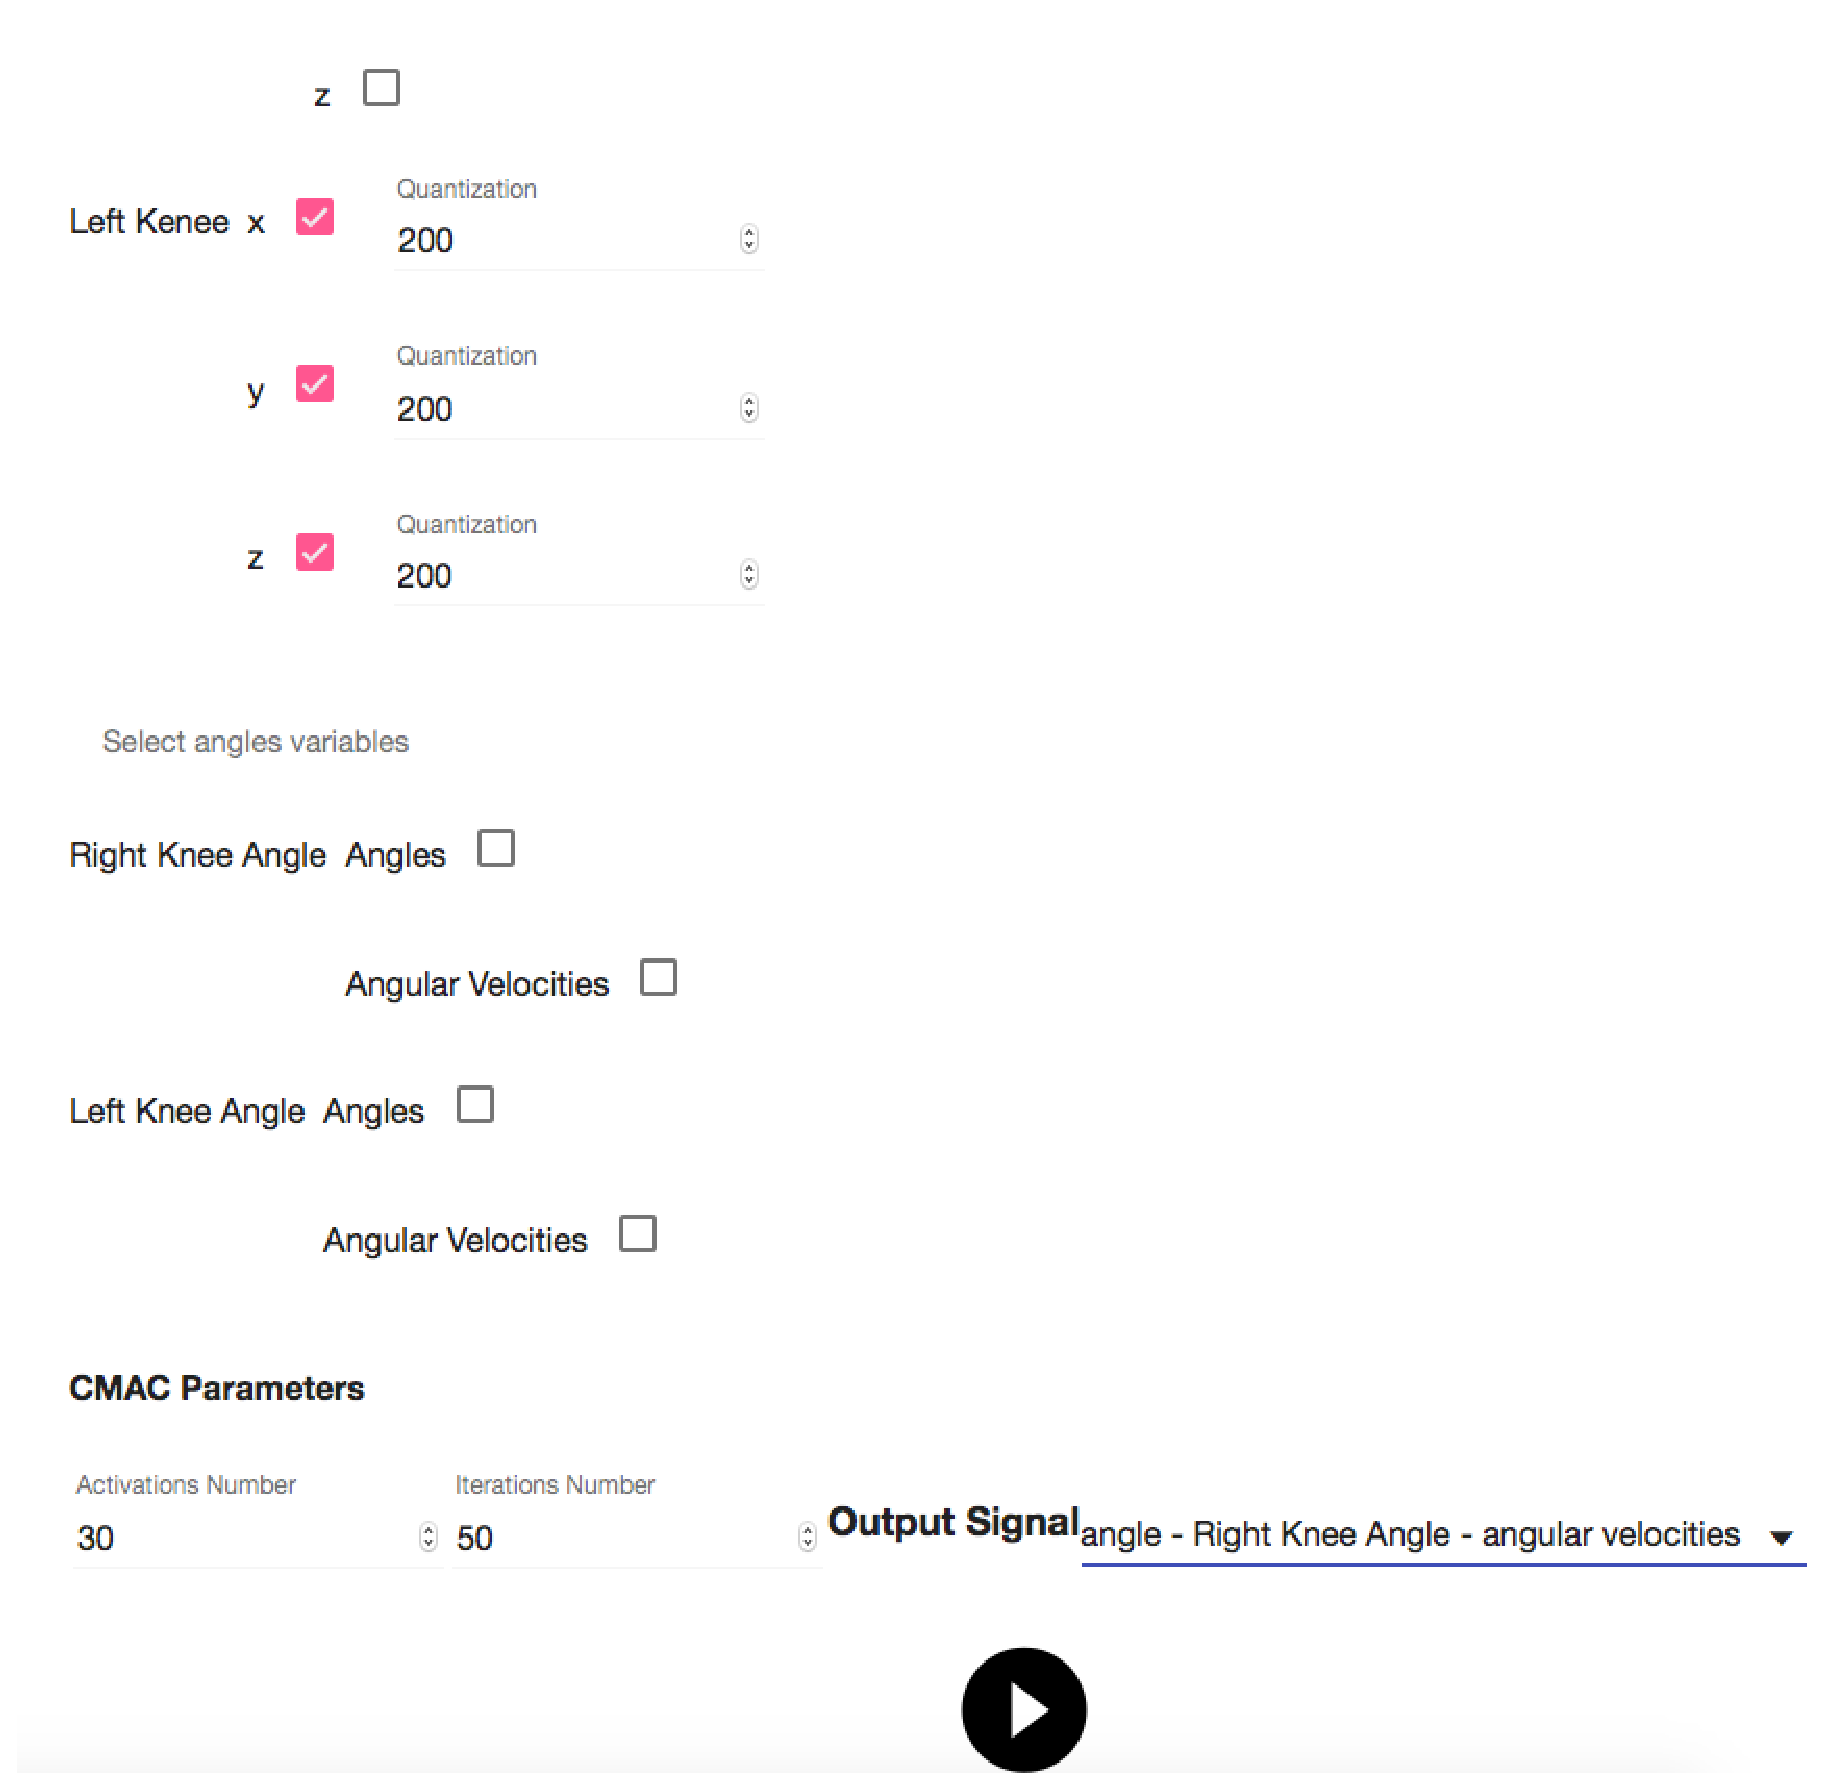
\includegraphics[width=10cm]{figuras/tela31.eps}
	\caption{Exemplo de configuração para uma simulação usando \emph{CMAC}.}
\label{tela31}
\end{figure}

\begin{figure}[H]
	\centering
	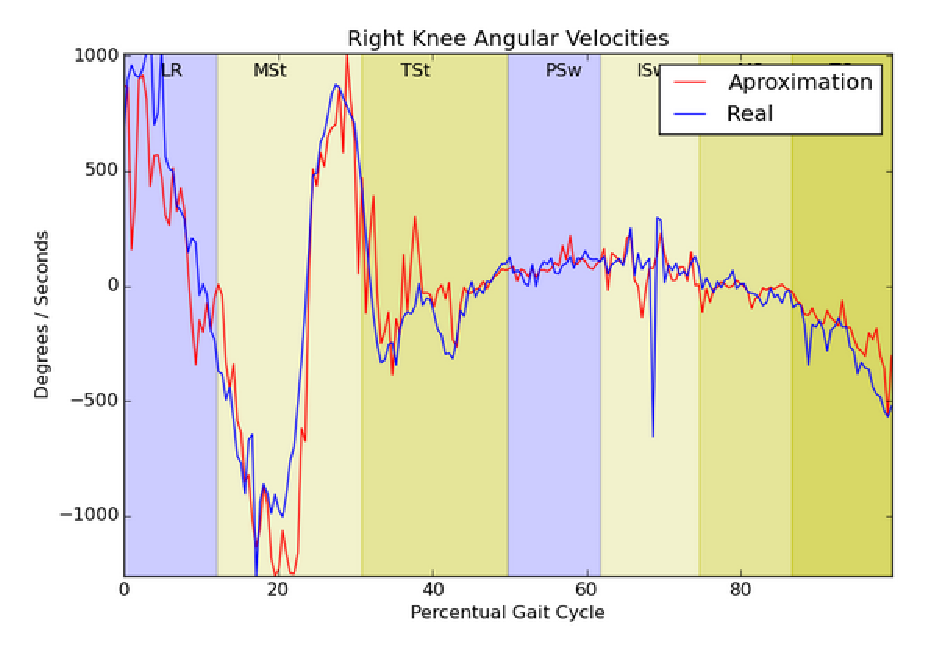
\includegraphics[width=10cm]{figuras/tela32.eps}
	\caption{Resultado da simulação.}
\label{tela32}
\end{figure}

\begin{figure}[H]
	\centering
	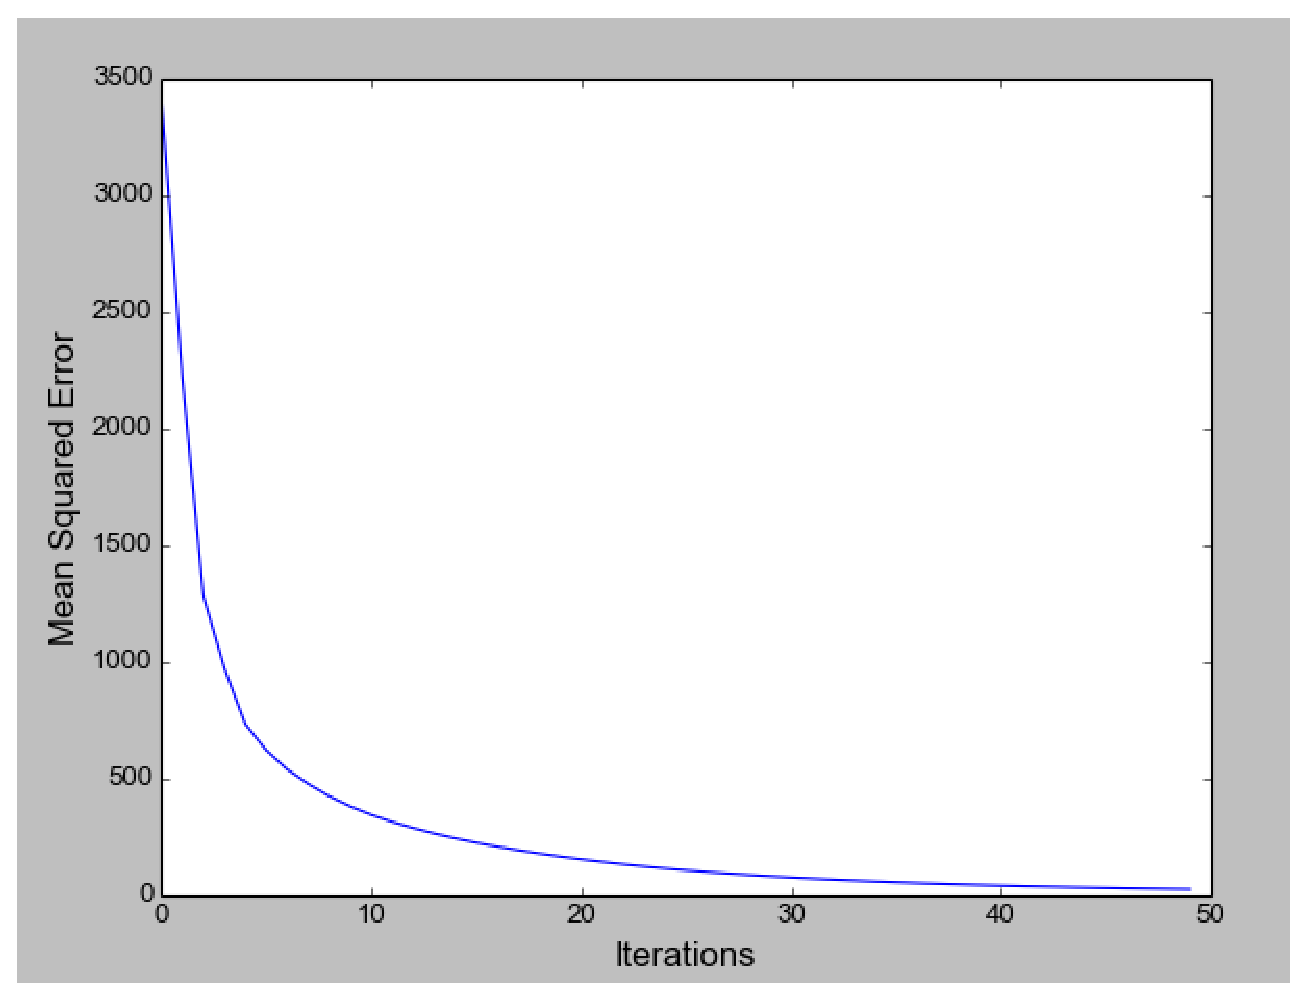
\includegraphics[width=10cm]{figuras/tela33.eps}
	\caption{Erro quadrado médio em cada iteração da simulação.}
\label{tela33}
\end{figure}

\section{Uso do sistema em dispositivos móveis}
Uma das maiores vantagens nas tecnologia escolhidas para compor a camada web, é sua total compatibilidade com dispositivos móveis capazes de executar \emph{browsers} modernos como \emph{Firefox, Chrome ou Safari}. O \emph{angular-material} já apresenta comportamentos muito bons em dispositivos de pequenas telas. 
Veja um exemplo nas Figuras \ref{tela34} e \ref{tela35} da aplicação rodando no \emph{browser} \emph{Firefox}, num dispositivo \emph{Motorola Xoom}. A Figura \ref{tela36} mostra a aplicação rodando em um \emph{iPhone4} com \emph{browser Safari}.

\begin{figure}[H]
	\centering
	\includegraphics[width=12cm]{figuras/tela34.eps}
	\caption{Aplicação \emph{Open Gait Analytics} rodando num \emph{browser Firefox} e dispositivo \emph{Motorola Xoom}.}
\label{tela34}
\end{figure}

\begin{figure}[H]
	\centering
	\includegraphics[width=12cm]{figuras/tela35.eps}
	\caption{Animação de uma amostra de marcha rodando num \emph{browser Firefox} e dispositivo \emph{Motorola Xoom}.}
\label{tela35}
\end{figure}

\begin{figure}[H]
	\centering
	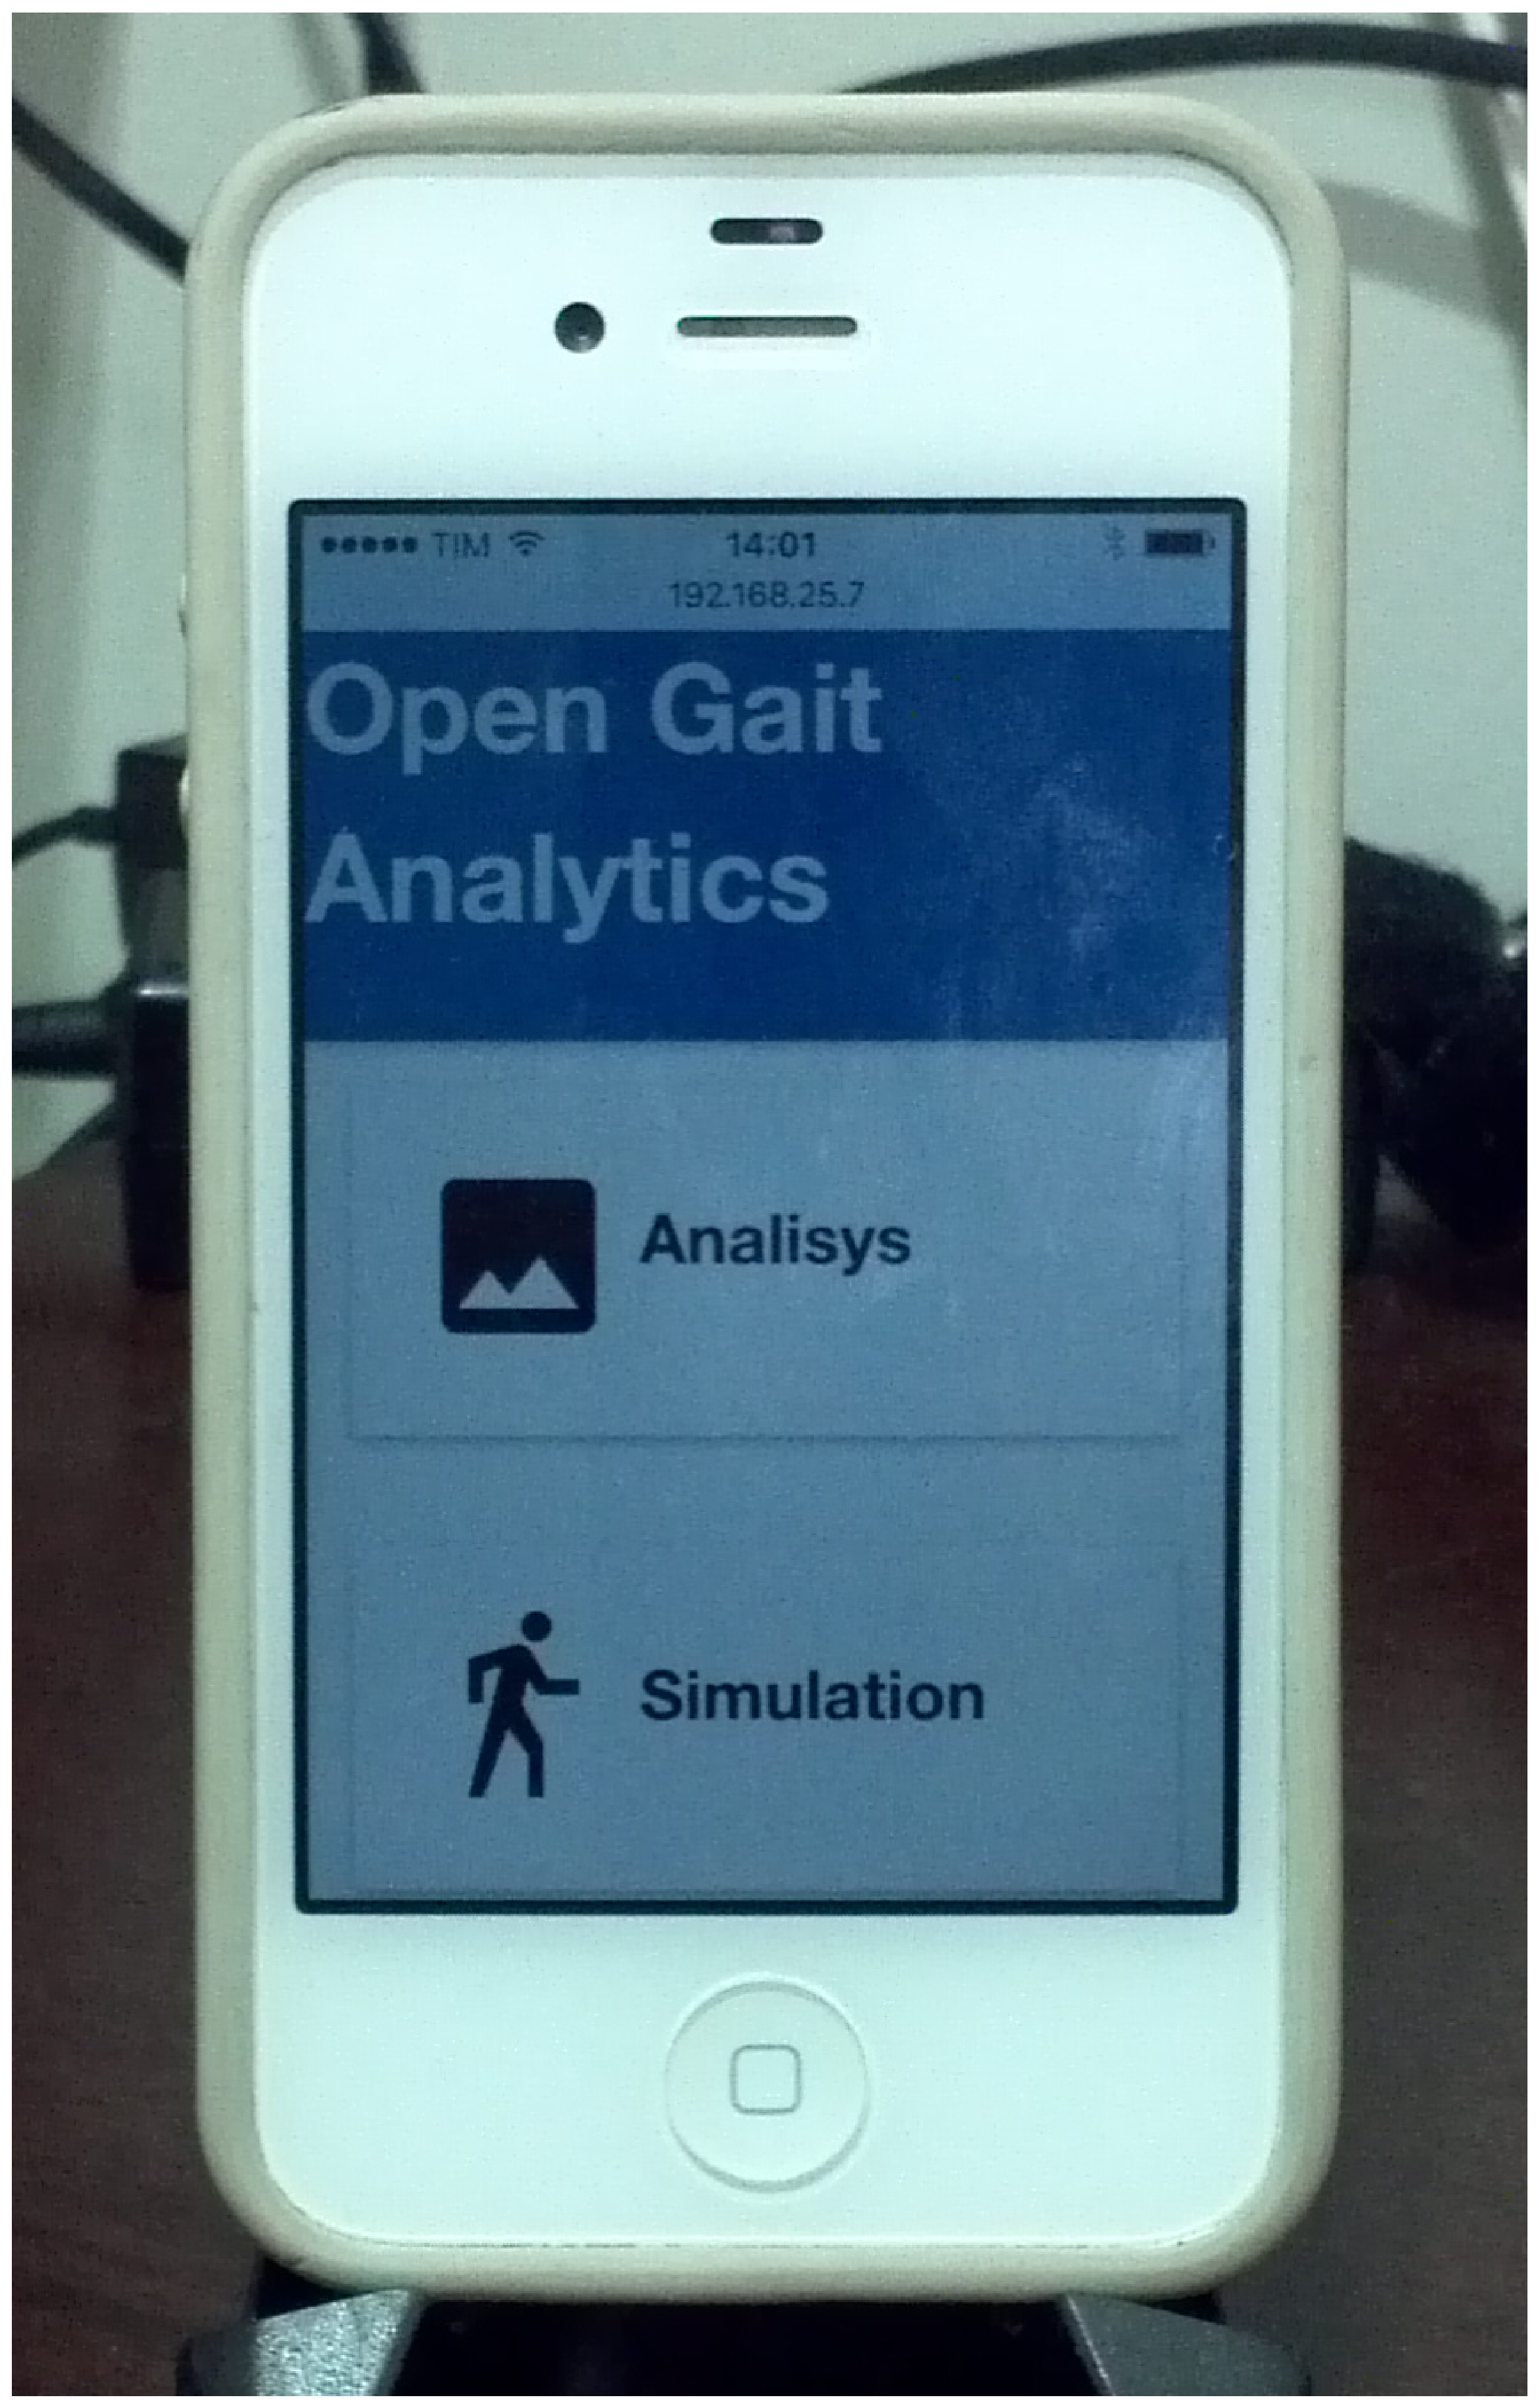
\includegraphics[width=5.5cm]{figuras/tela36.eps}
	\caption{Aplicação rodando num \emph{iPhone 4} com \emph{browser Safari}.}
\label{tela36}
\end{figure}


Para frisar como a aplicação se adapta inteligentemente ao dispositivo que está rodando, compare a Figura \ref{tela34} com a Figura \ref{comp1}. 
Veja que a barra lateral desaparece na tela menor do \emph{iPhone 4}. Em cima da tela aparece a opção \emph{open side} que quando clicada mostra a barra lateral por cima do formulário.
\begin{figure}[H]
  \centering
  \begin{minipage}[b]{0.35\textwidth}
    \includegraphics[width=\textwidth]{figuras/tela37.eps}
  \end{minipage}
  \hfill
  \begin{minipage}[b]{0.35\textwidth}
    \includegraphics[width=\textwidth]{figuras/tela38.eps}
  \end{minipage}
  \caption{Adaptação da aplicação em telas pequenas.}
  \label{comp1}
\end{figure}


Para o profissional de saúde, este é um recurso a mais, pois agora do seu próprio celular e em qualquer lugar ele poder ver dados dos seus pacientes.

